\documentclass[12pt]{beamer}
\usepackage{algorithm2e} %pseudocodigos
\usepackage{algorithmic} %pseudocodigos
\usepackage{float}
\usepackage{xmpmulti}
\usetheme{Berkeley}
\usepackage{animate}
%\usepackage{movie15}
\usepackage{graphicx}
\graphicspath{{imagens/}}
\usepackage{booktabs}
\usepackage[english]{babel}
\usepackage{pgfpages}


%opções de para comentarios ao lado da tela
%\setbeameroption{hide notes} % Only slides
%\setbeameroption{show only notes} % Only notes
%\setbeameroption{show notes on second screen}
%\setbeameroption{second mode text on second screen=⟨screen⟩}
%\setbeameroption{show notes on second screen=right} % Both

%\logo{\includegraphics[height=1cm]{example-image-c}}
%\logo{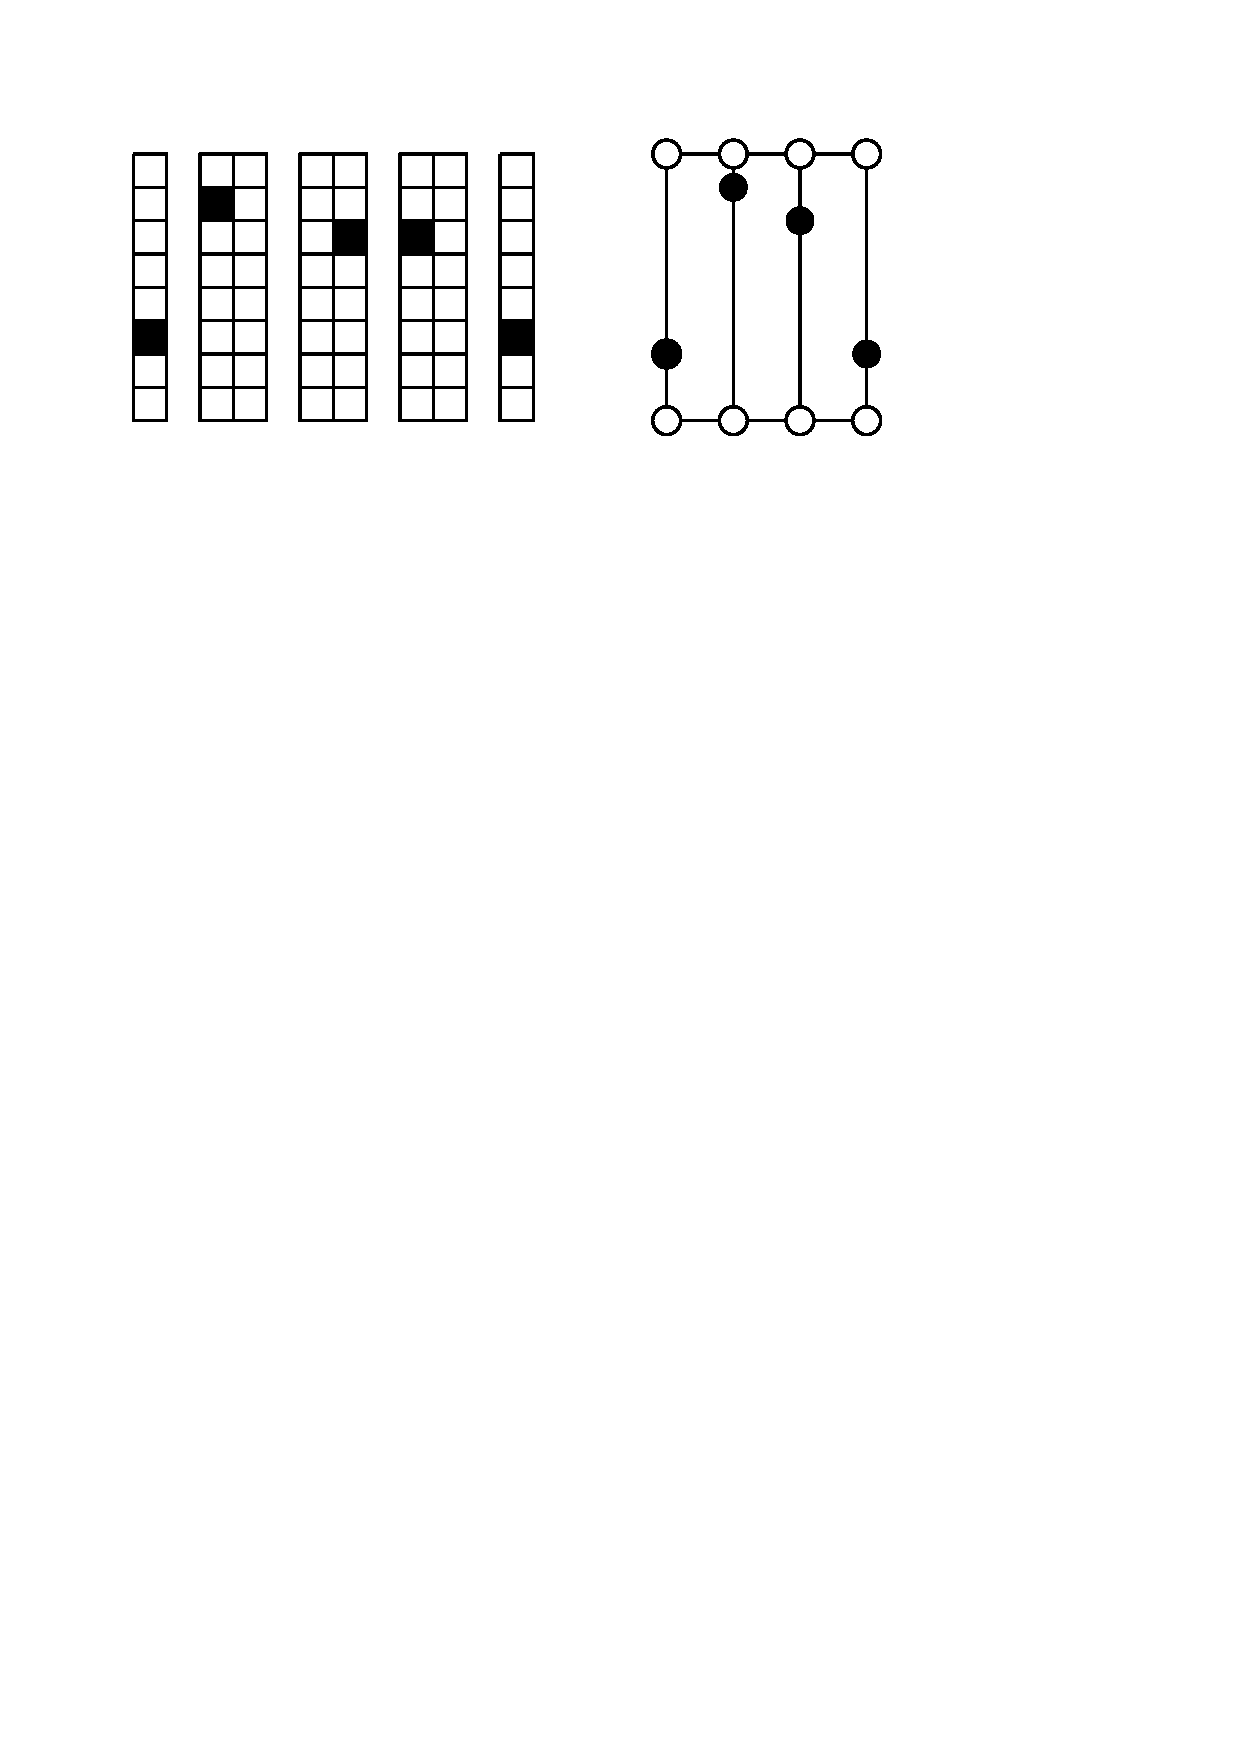
\includegraphics[height=1cm]{CD_1}}
\logo{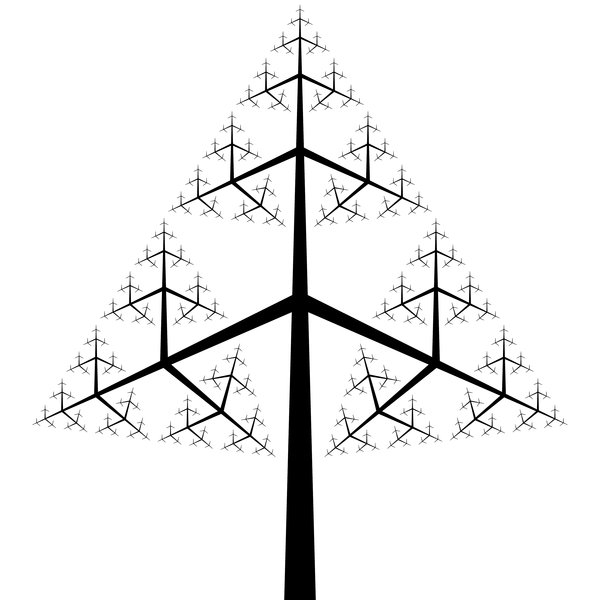
\includegraphics[width=0.20\linewidth]{imagens/logo}}
\title[]{Uma nova heur\'istica para o "Single-Picker-Routing-Problem" com restri\c{c}\~oes pr\'aticas de carregamento}



\author{Alexandre Checoli Choueiri}
\institute[AI]
{UFPR  \\ % Your institution for the title page
	\medskip
	\textit{alexandrechecoli@gmail.com} % Your email address
	
}
\date{\today}

\begin{document}
	
	\begin{frame} 
		\titlepage % Print the title page as the first slide	
	\end{frame}
	
	\begin{frame}{Sum\'ario}
		\tableofcontents
	\end{frame}
		
	
\section{Motiva\c{c}\~ao}
%%%%%%%%%%%%%%%%%%%%%%%%%%%%%%%%%%%%%%%%%%%%%%%%%%%%%%%%%%%%%%%%%%%%%%%%%%%%%%%%%%
\begin{frame}{Motiva\c{c}\~ao}
	
	\begin{enumerate}
		\item {\bfseries Fidedignidade :}	
		Estudos na \'area de Roteamento em \'armazens carecem de Fidedignidade, ao considerarem somente aspectos relacionados \'a rota.
	\end{enumerate}
	\begin{enumerate}
		\item {\bfseries Depend\^encia de Solvers :}	
		Muitas das solu\c{c}\~oes tratadas na literatura dependem de Softwares comerciais para que os modelos sejam otimizados.
	\end{enumerate}	
\end{frame}

\section{Objetivos}
%%%%%%%%%%%%%%%%%%%%%%%%%%%%%%%%%%%%%%%%%%%%%%%%%%%%%%%%%%%%%%%%%%%%%%%%%%%%%%%%%%
\begin{frame}{Objetivos}

	\begin{itemize}
		\item{Estudar o modelo matematico de Scholz, adapatando-o para um m\'etodo heur\'istico}
		\pause	
		\item{A adapatar a Heur\'istica com restri\c{c}\~oes de carregamento:}
		\begin{itemize}
			\item{Estabilidade vertical}
			\item{Empilhamento m\'aximo} 
		\end{itemize}
		\pause
		\item{Respeitando a pol\'itica L.I.F.O para coleta dos itens}
	\end{itemize}
\end{frame}



%%%%%%%%%%%%%%%%%%%%%%%%%%%%%%%%%%%%%%%%%%%%%%%%%%%%%%%%%%%%%%%%%%%%%%%%%%%%%%%%%%
\section{Descri\c{c}\~ao do problema (SPRP)}
	\begin{frame}{Descri\c{c}\~ao do problema}
	\framesubtitle{Original (SPRP)}	
		Definir a rota em em um armaz\'em,de tal forma a visitar todos os pontos de coleta:
			\begin{figure}
			\pause
			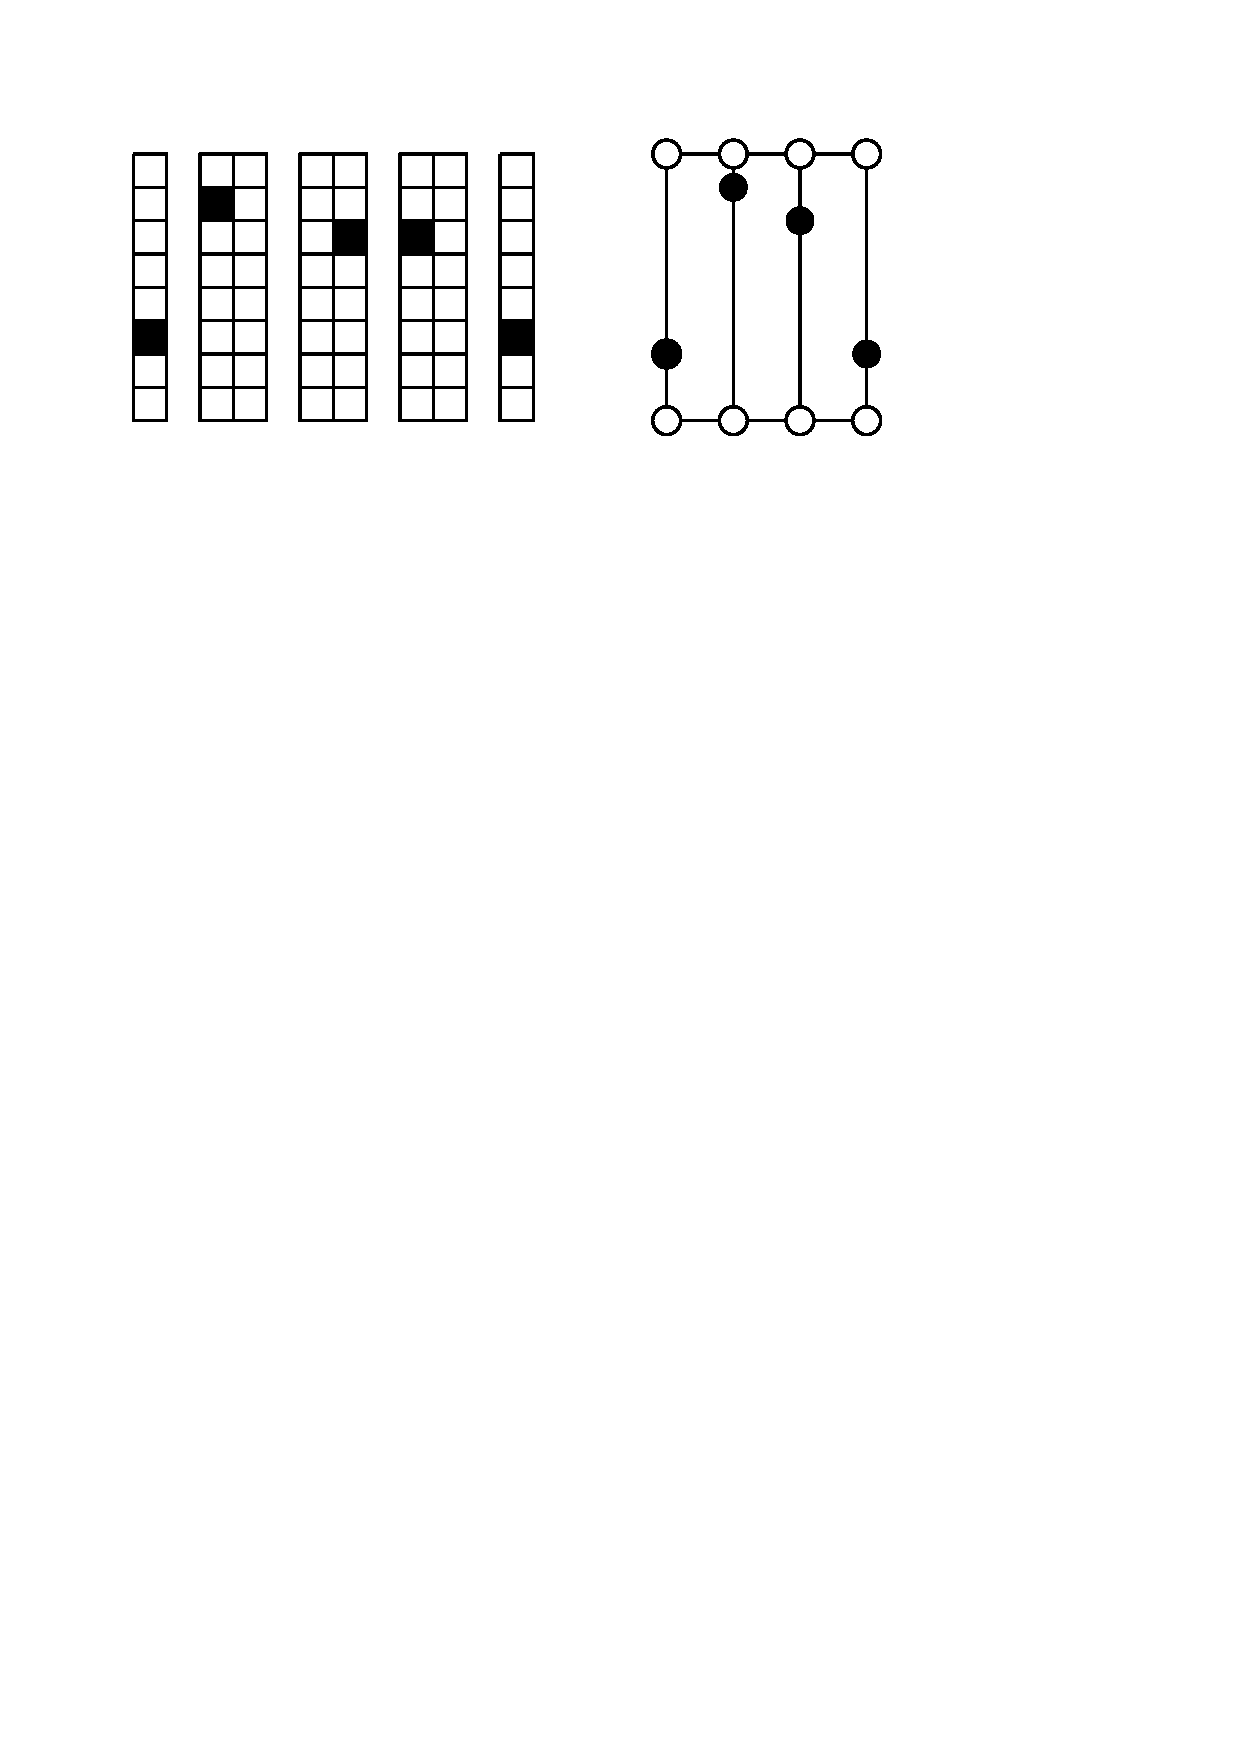
\includegraphics[width=1\linewidth]{CD_1}
			\caption{Representa\c{c}\~ao de armaz\'em via grafo}
			
		\end{figure}
	\pause
	\begin{itemize}
		\item {\bfseries Problema :}
		Infactibilidade da rota devido ao sobrevolume do palete
	\end{itemize}
	\end{frame}


%Frame dividido na tela
\begin{frame}{Descri\c{c}\~ao do problema}
	\framesubtitle{(CSPRP)}
\fboxsep=0pt
\noindent{%
	\begin{minipage}[t]{0.48\linewidth}
		\begin{itemize}
		\item[]
		\item \bfseries{Localiza\c{c}\~ao Geometrica das caixas}
		\item[] %itemize que esconde o bullet, só para o posicionamento ficar correto na imagem
		\item[]
		\item[]
		%\item \bfseries{Restri\c{c}\~oes de empilhamento m\'aximo das caixas}
		\end{itemize}

	\end{minipage}}%
\hfill%
{%
	\begin{minipage}[t]{0.48\linewidth}
		\begin{figure}			
			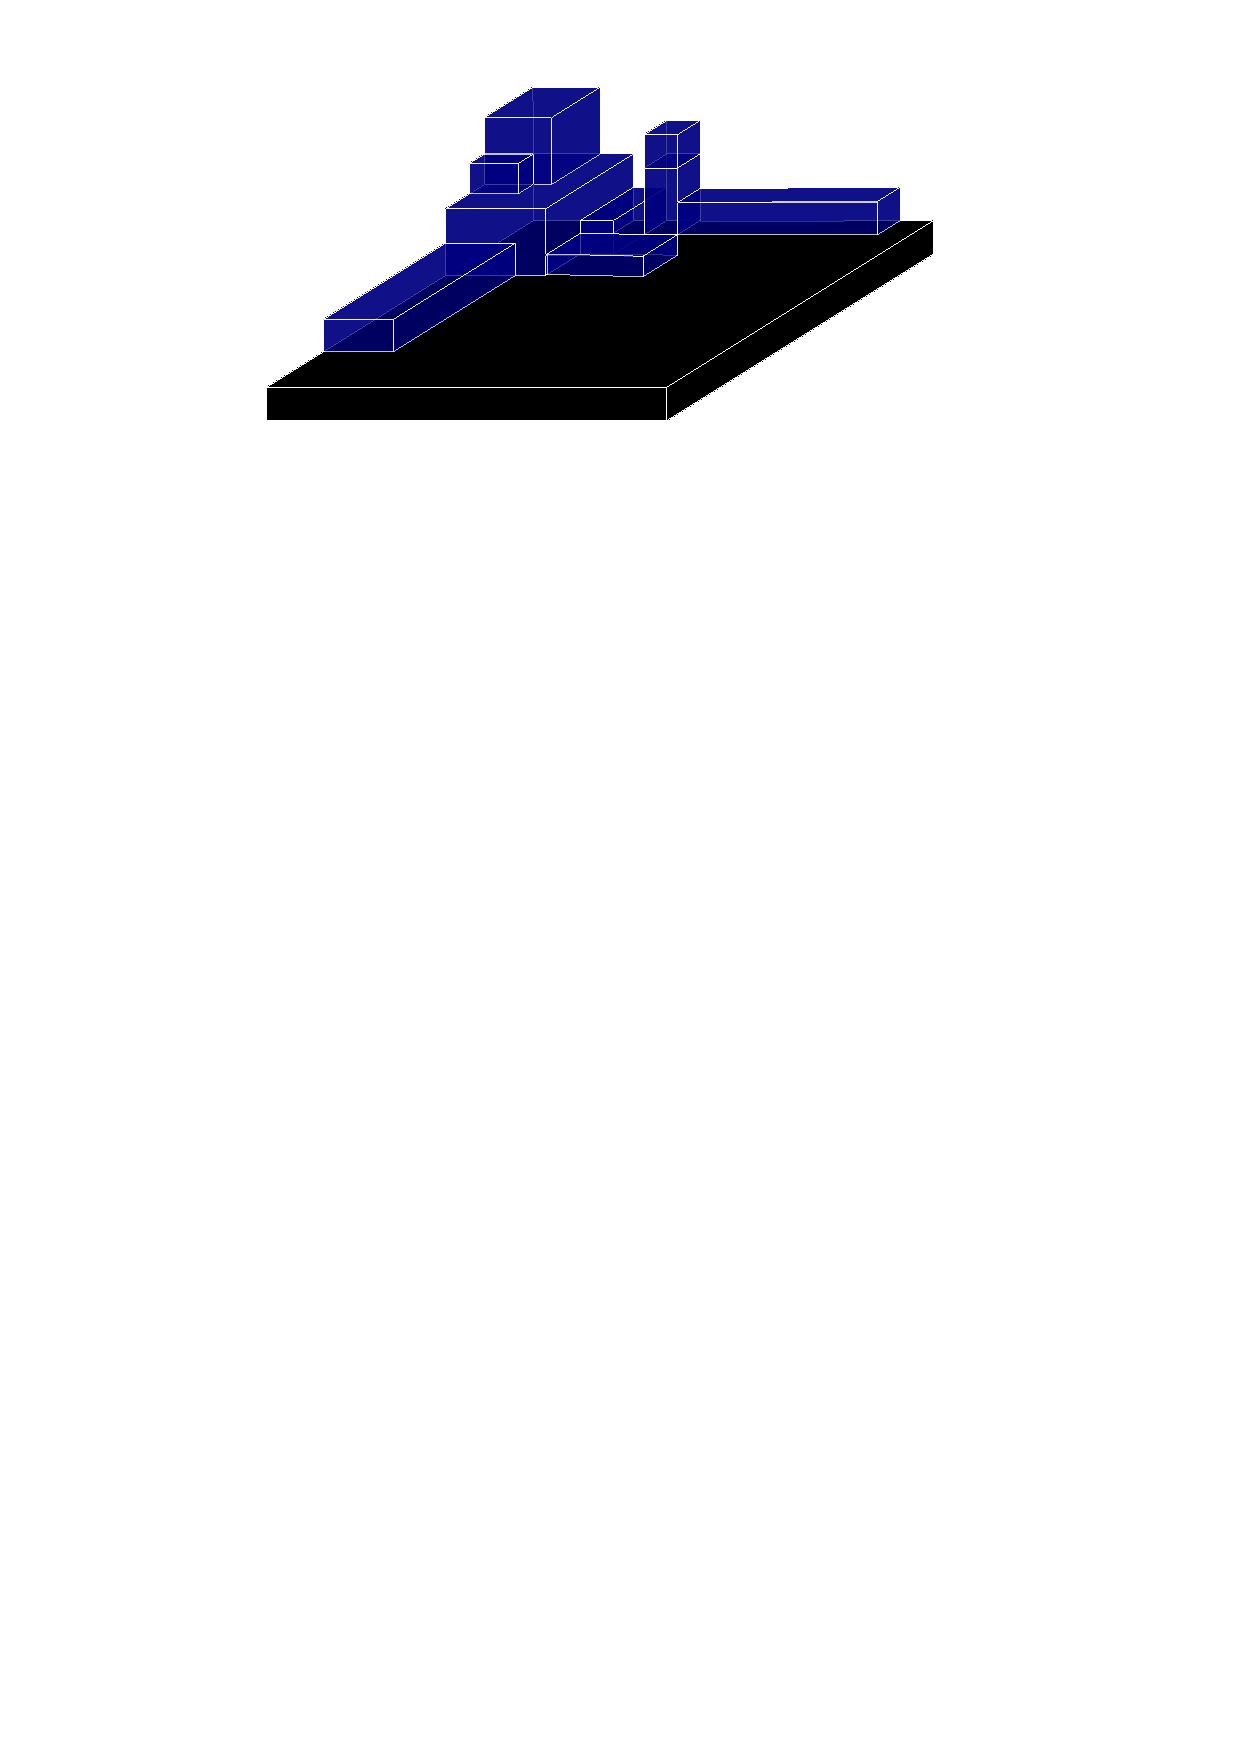
\includegraphics[width=1\linewidth]{volume_caixas}
		\end{figure}
		

	\end{minipage}
}
\end{frame}

\begin{frame}{Descri\c{c}\~ao do problema}
	\framesubtitle{(CSPRP)}
	\fboxsep=0pt
	\noindent{%
		\begin{minipage}[t]{0.48\linewidth}
			\begin{itemize}
				\item[]
				\item \bfseries{Localiza\c{c}\~ao Geometrica das caixas}
				\item[] %itemize que esconde o bullet, só para o posicionamento ficar correto na imagem
				\item[]
				\item[]
				\item \bfseries{Restri\c{c}\~oes de empilhamento m\'aximo das caixas}
			\end{itemize}
			
	\end{minipage}}%
	\hfill%
	{%
		\begin{minipage}[t]{0.48\linewidth}
			\begin{figure}			
				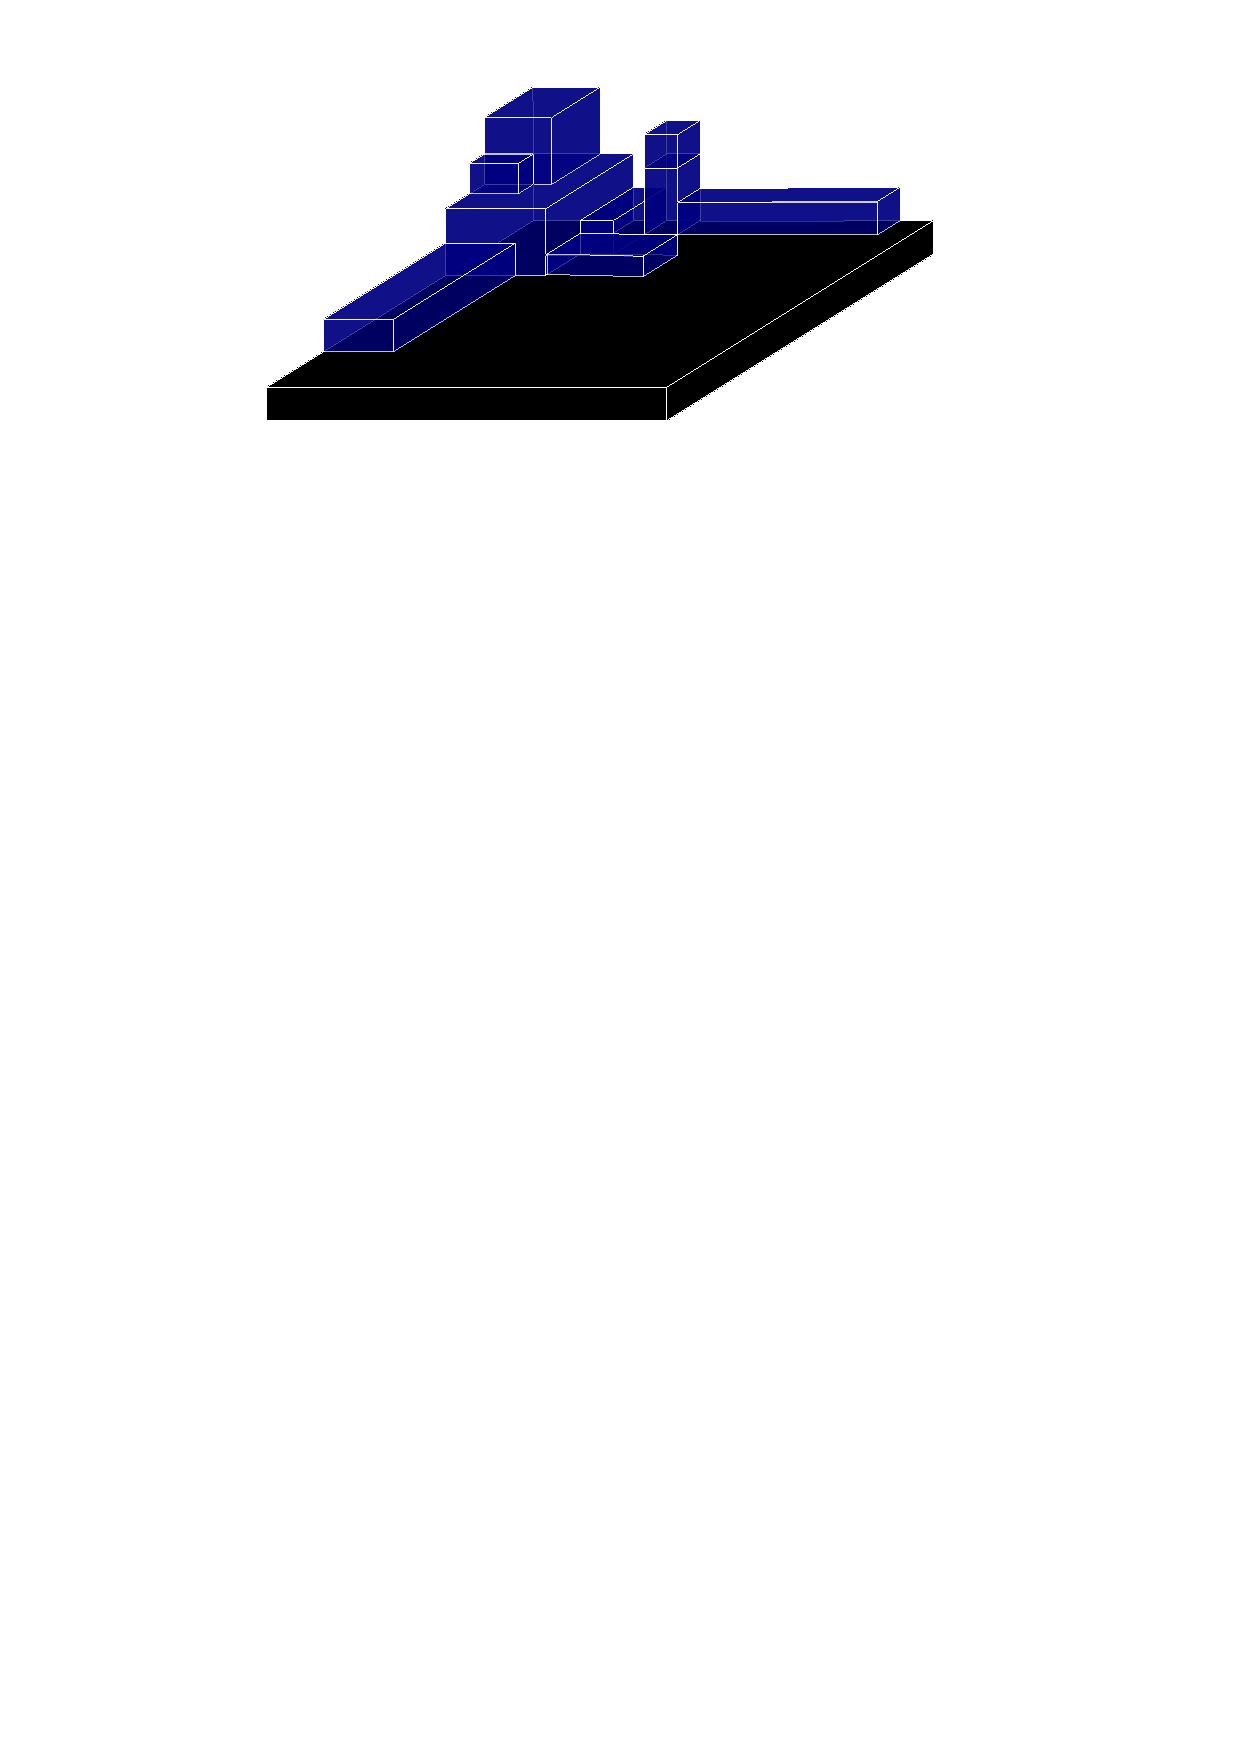
\includegraphics[width=1\linewidth]{volume_caixas}
			\end{figure}
			\begin{figure}			
				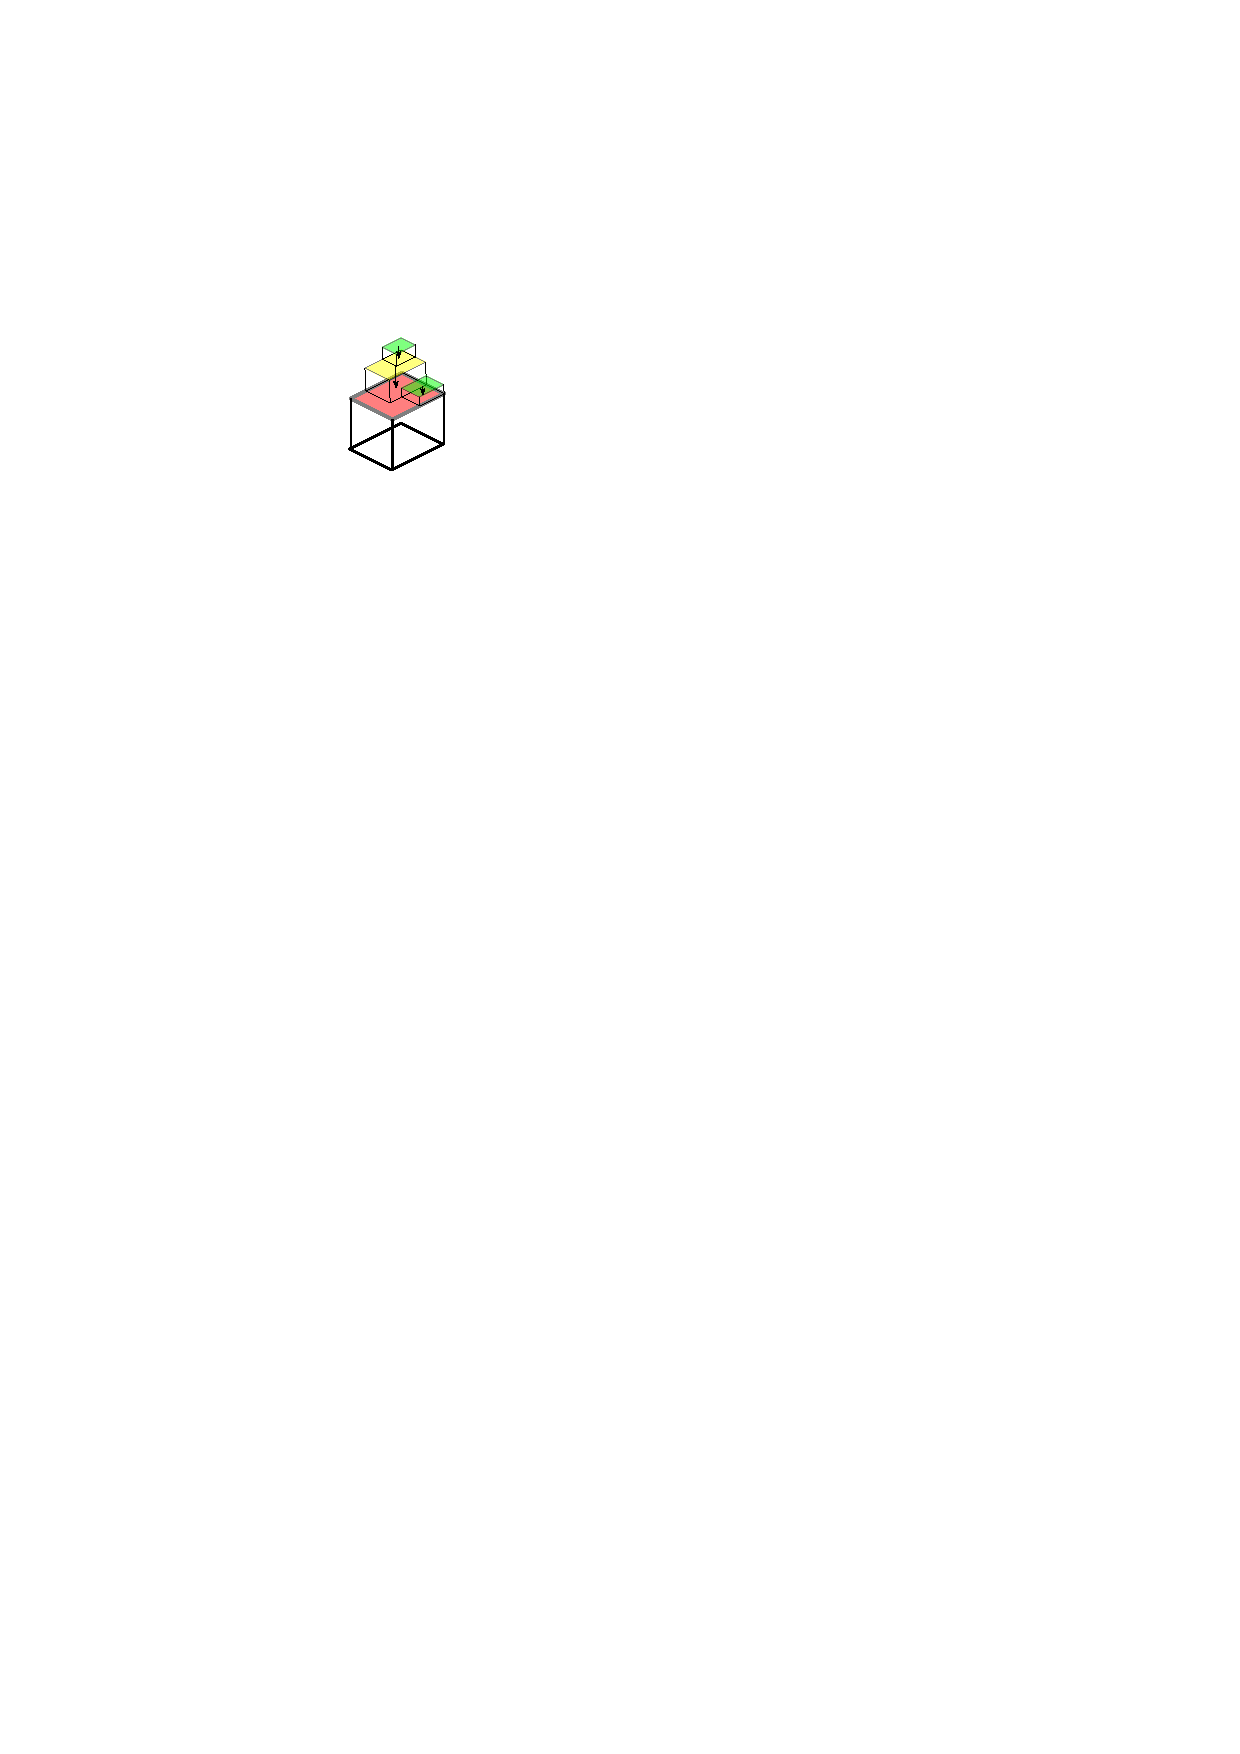
\includegraphics[width=0.45\linewidth]{pressao_caixas}
				
			\end{figure}
		\end{minipage}
	}
\end{frame}

\begin{frame}{Descri\c{c}\~ao do problema}
	\framesubtitle{(CSPRP)}
	\fboxsep=0pt
	\noindent%
		\begin{minipage}[t]{0.60\linewidth}
			\begin{itemize}
				\item[]
				\item {{Determinar um {\bfseries conjunto}} de rotas, tais que:
					\begin{itemize}
						\item todos os itens sejam coletados 
						\item n\~ao exista sobreposi\c{c}\~ao de caixas no palete
						\item o custo total das rotas seja o m\'inimo poss\'ivel  
					\end{itemize}}
				 
				 
		         
			\end{itemize}
			
	\end{minipage}%
	\hfill%
	{%
		\begin{minipage}[t]{0.35\linewidth}
			\pause
			\begin{figure}			
				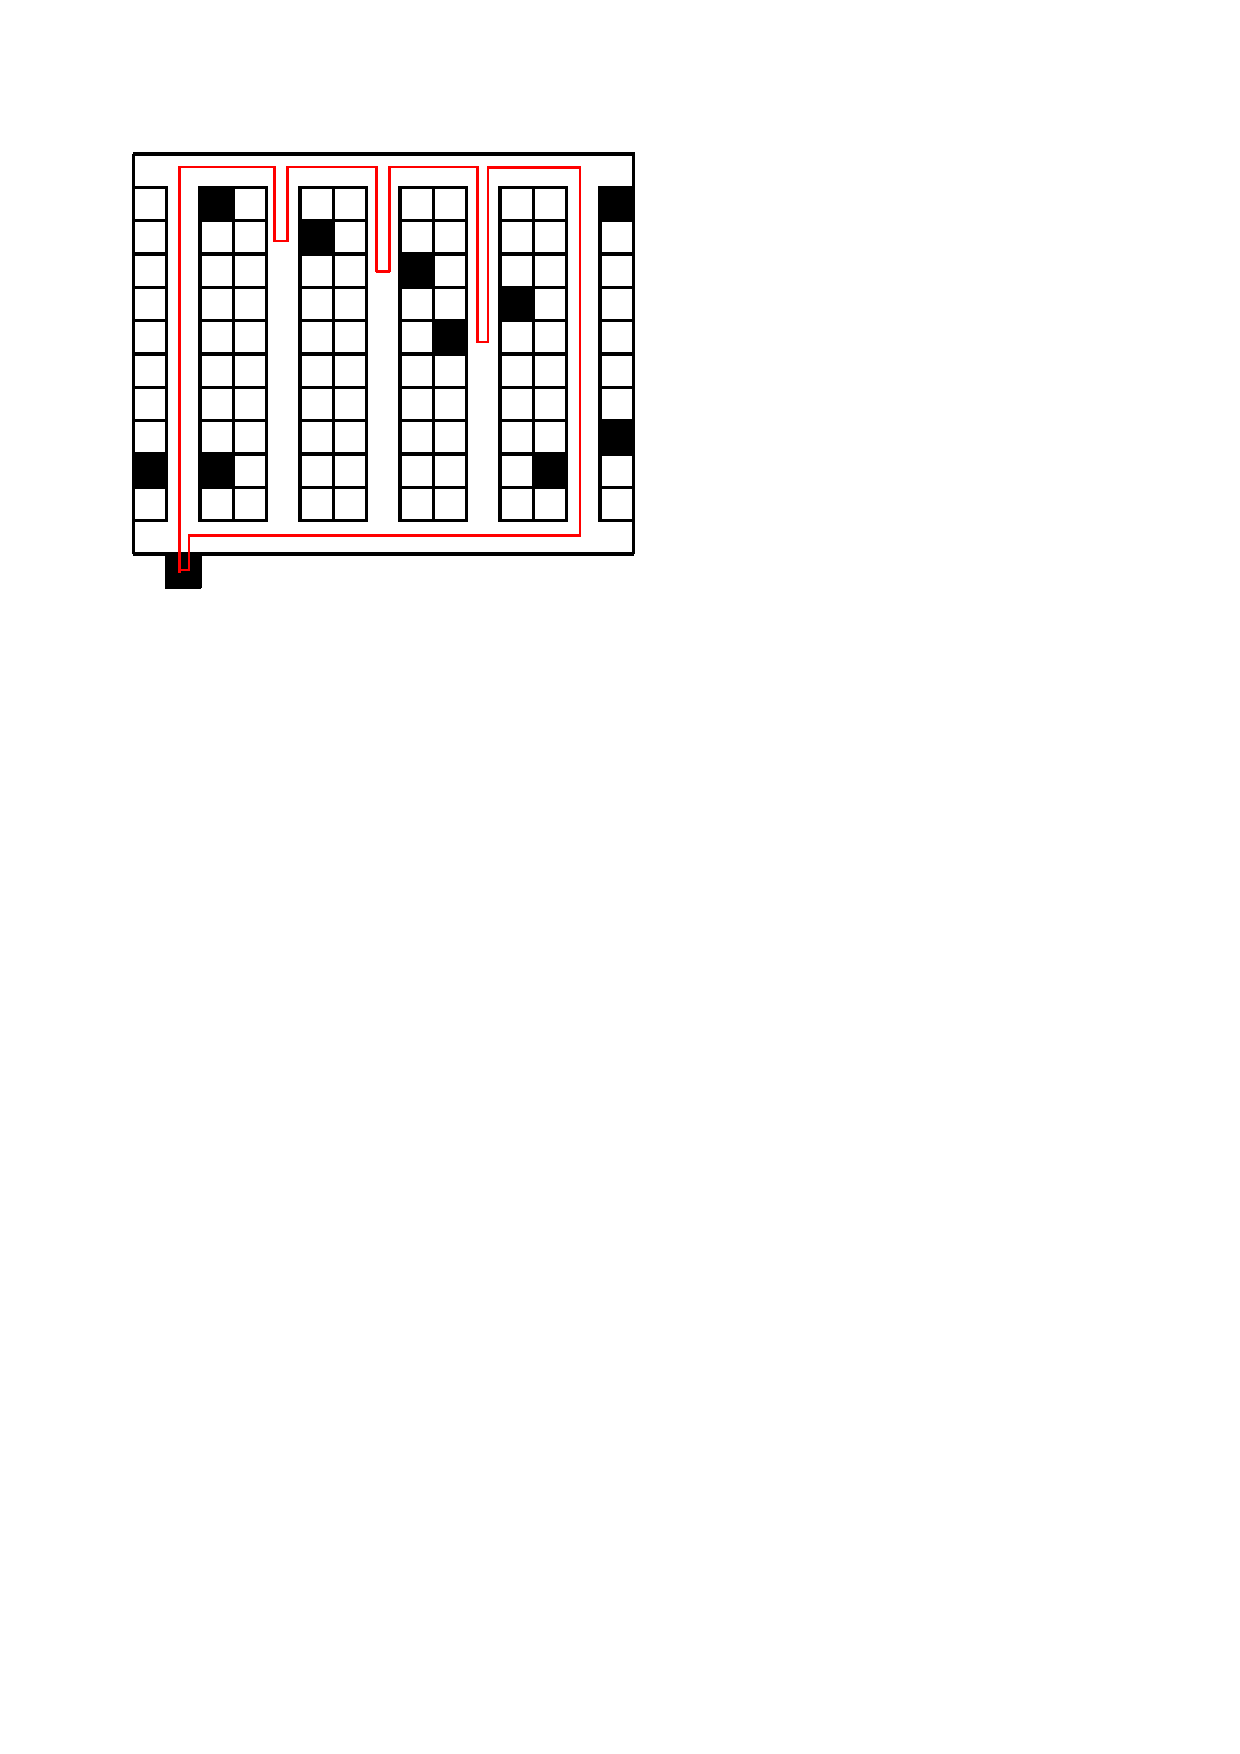
\includegraphics[width=0.9\linewidth]{rota_sprp}
			\end{figure}
		    \pause
			\begin{figure}			
				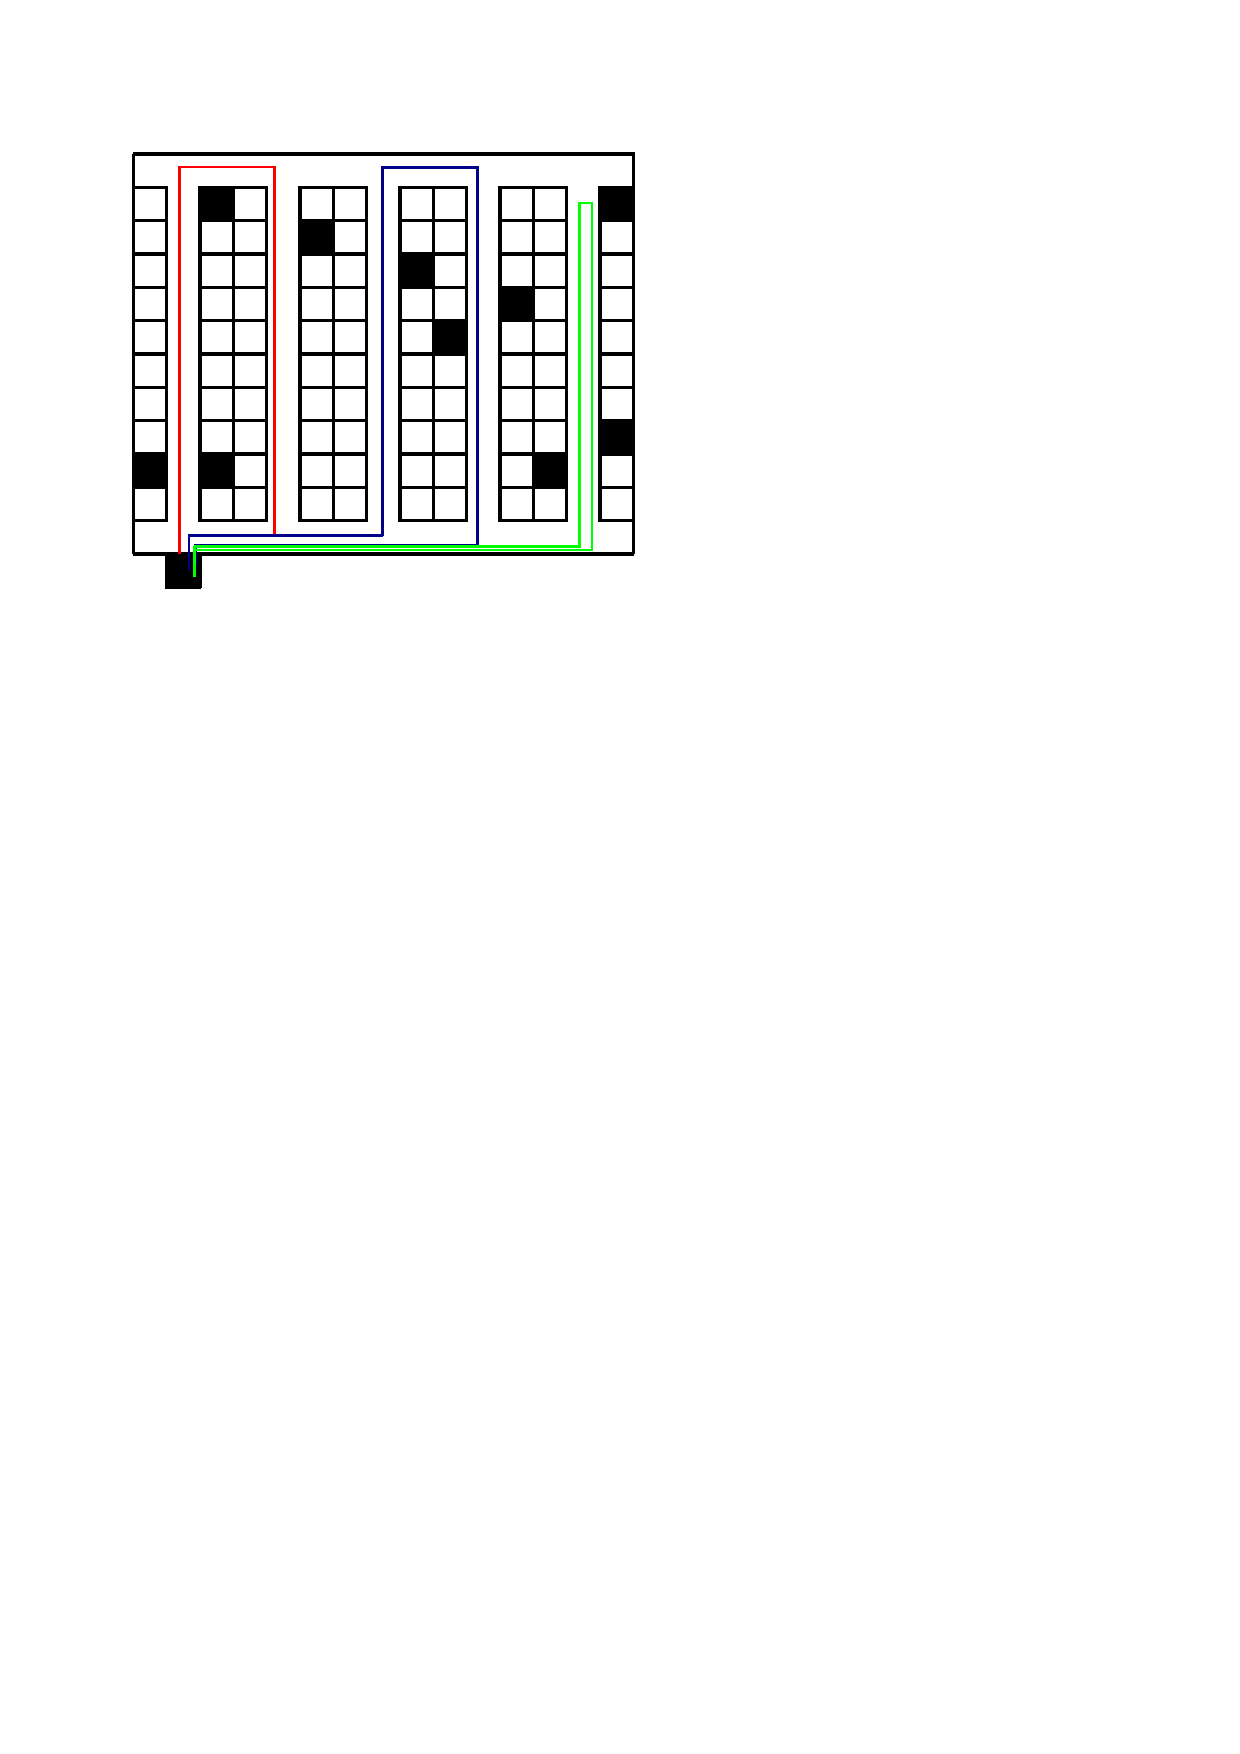
\includegraphics[width=0.9\linewidth]{rota_csprp}				
			\end{figure}
		\end{minipage}
	}
\end{frame}


%%%%%%%%%%%%%%%%%%%%%%%%%%%%%%%%%%%%%%%%%%%%%%%%%%%%%%%%%%%%%%%%%%%%%%%%%%%%%%%%%%
\section{Heur\'istica de corre\c{c}\~ao de rotas} %

	\begin{frame}{Heur\'istica de corre\c{c}\~ao de rotas}

	\framesubtitle{(Discretiza\c{c}\~ao de pontos (SCHOLZ, et al. 2016))}
	\fboxsep=0pt
	\noindent\fbox{%
		\begin{minipage}[t]{0.48\linewidth}
			\begin{itemize}
				\item[]
			\end{itemize}
		\begin{figure}			
			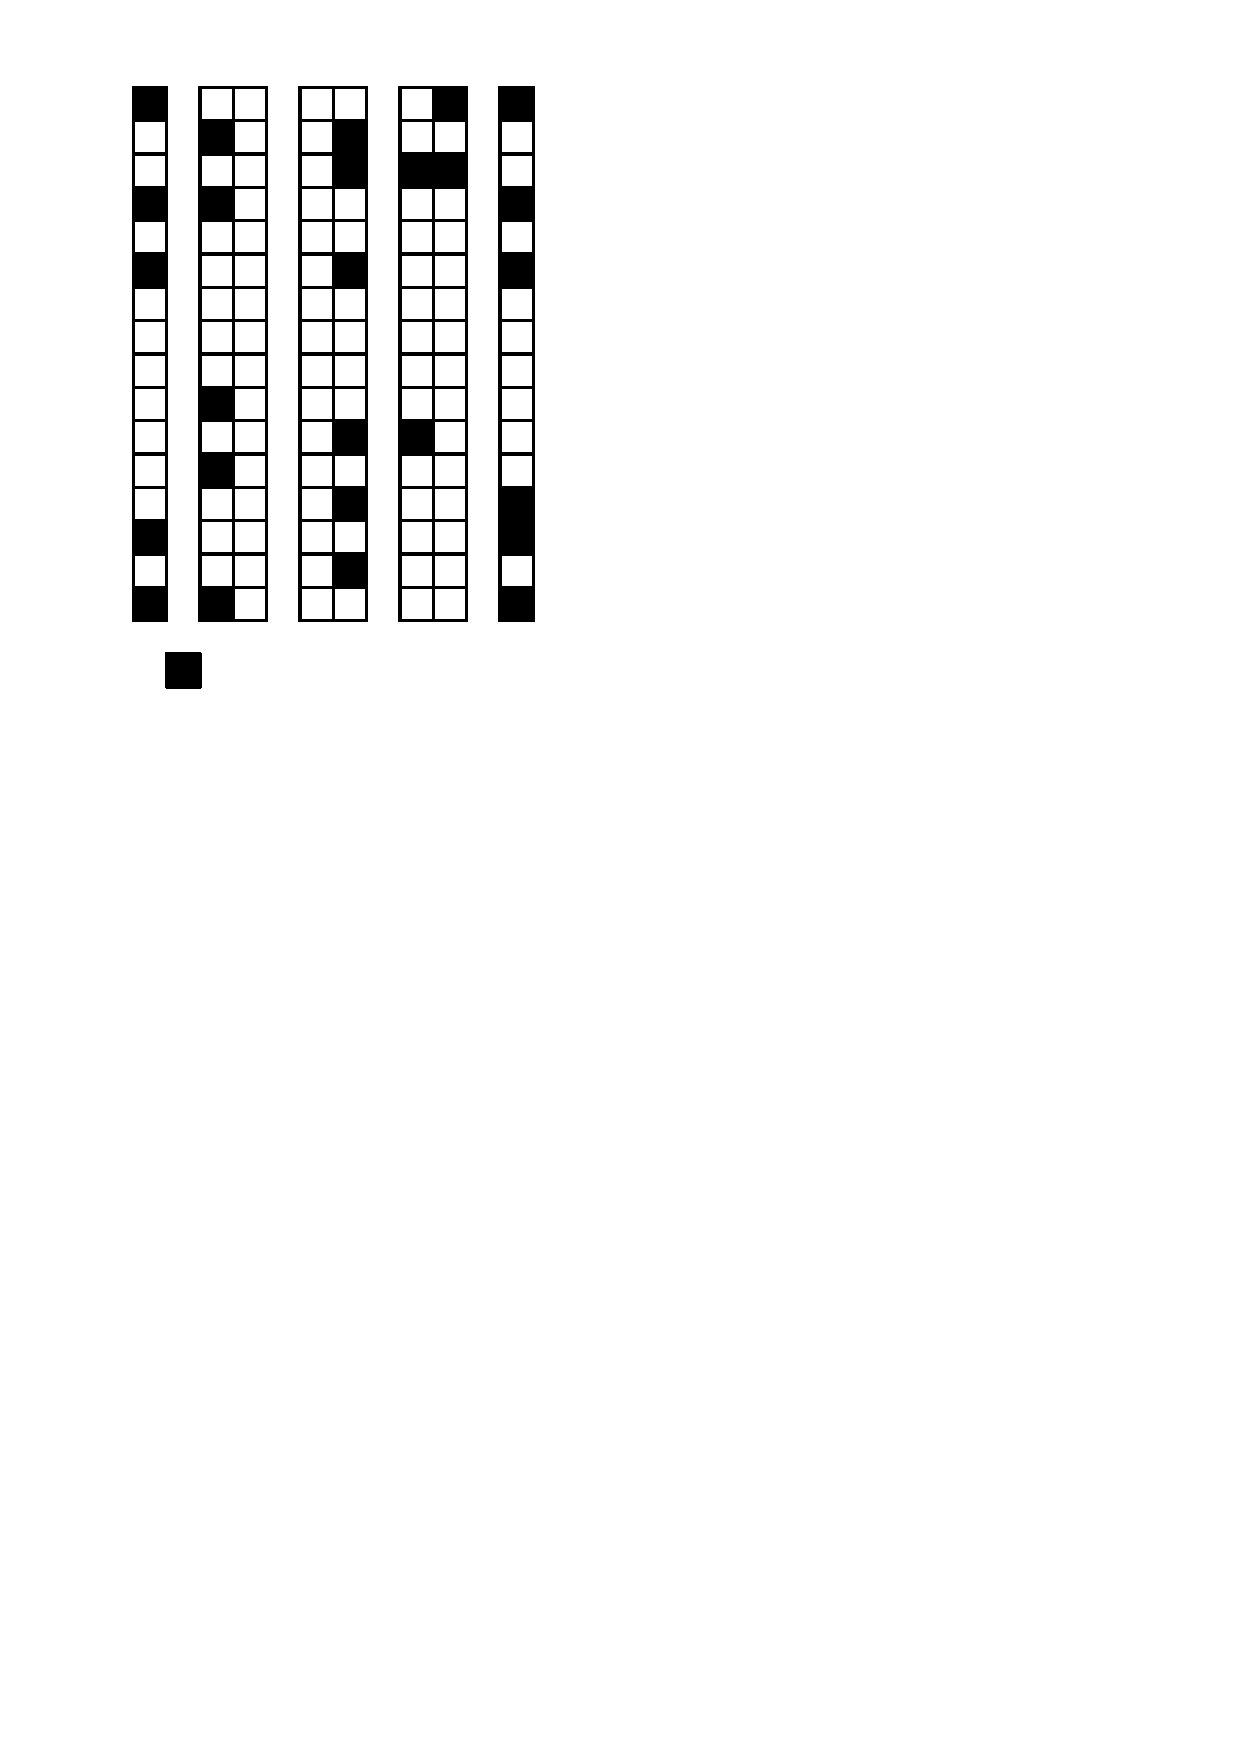
\includegraphics[width=0.8\linewidth]{discret_1}
		\end{figure}

			\end{minipage}}%
		\hfill%
	{%
		\noindent\fbox{%
		\begin{minipage}[t]{0.48\linewidth}

		
		\end{minipage}}}%
		\hfill%
		
	\end{frame}
	\begin{frame}{Heur\'istica de corre\c{c}\~ao de rotas}
	\framesubtitle{(Discretiza\c{c}\~ao de pontos (SCHOLZ, et al. 2016))}
	\fboxsep=0pt
	Redu\c{c}\~ao no n\'umero de pontos para coleta
	\noindent\fbox{%
		\begin{minipage}[t]{0.48\linewidth}
			\begin{itemize}
				\item[] {\small 26 pontos}
			\end{itemize}
			\begin{figure}			
				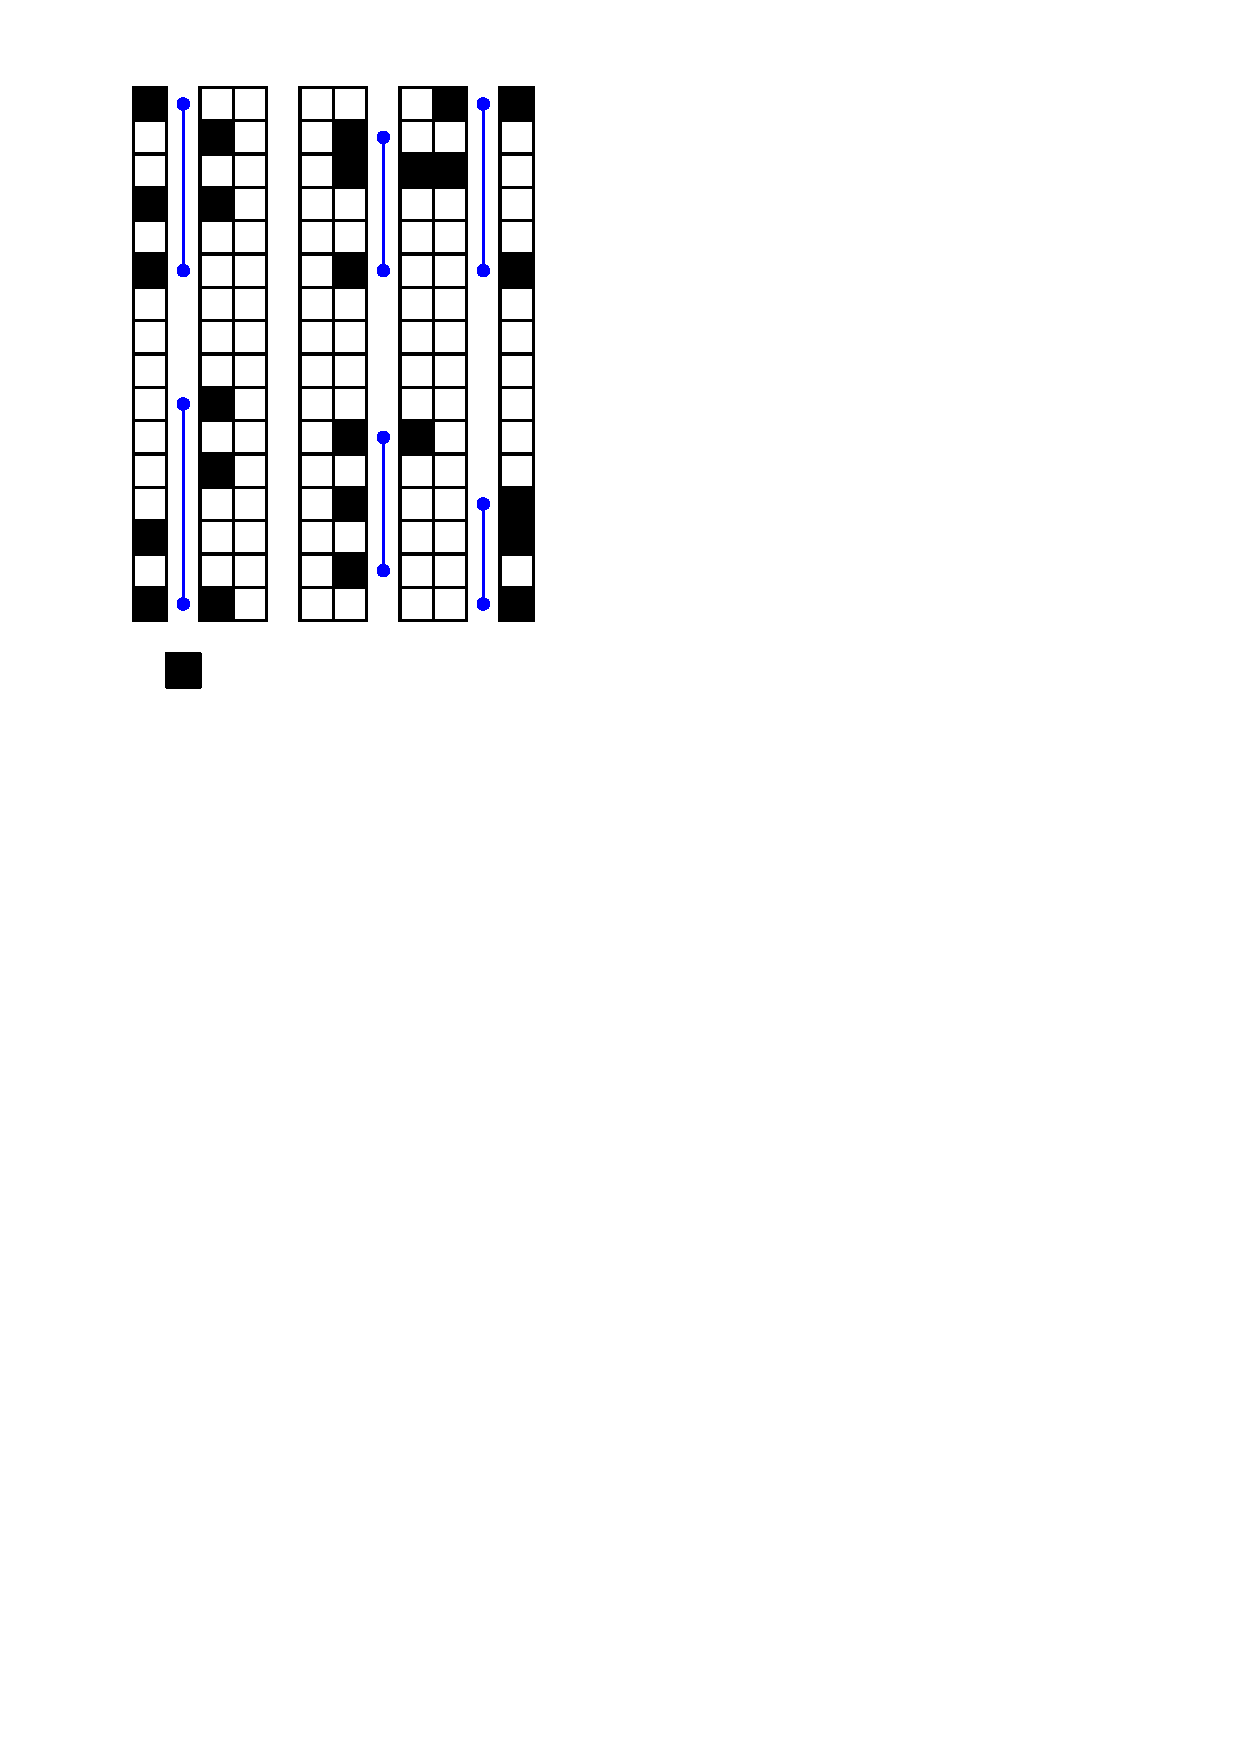
\includegraphics[width=0.8\linewidth]{discret_4}
			\end{figure}
			
	\end{minipage}}%
	\hfill%
	{%
		\noindent\fbox{%
			\pause
			\begin{minipage}[t]{0.48\linewidth}
				\begin{itemize}
					\item[] {\small 12 pontos}
				\end{itemize}
				\begin{figure}			
					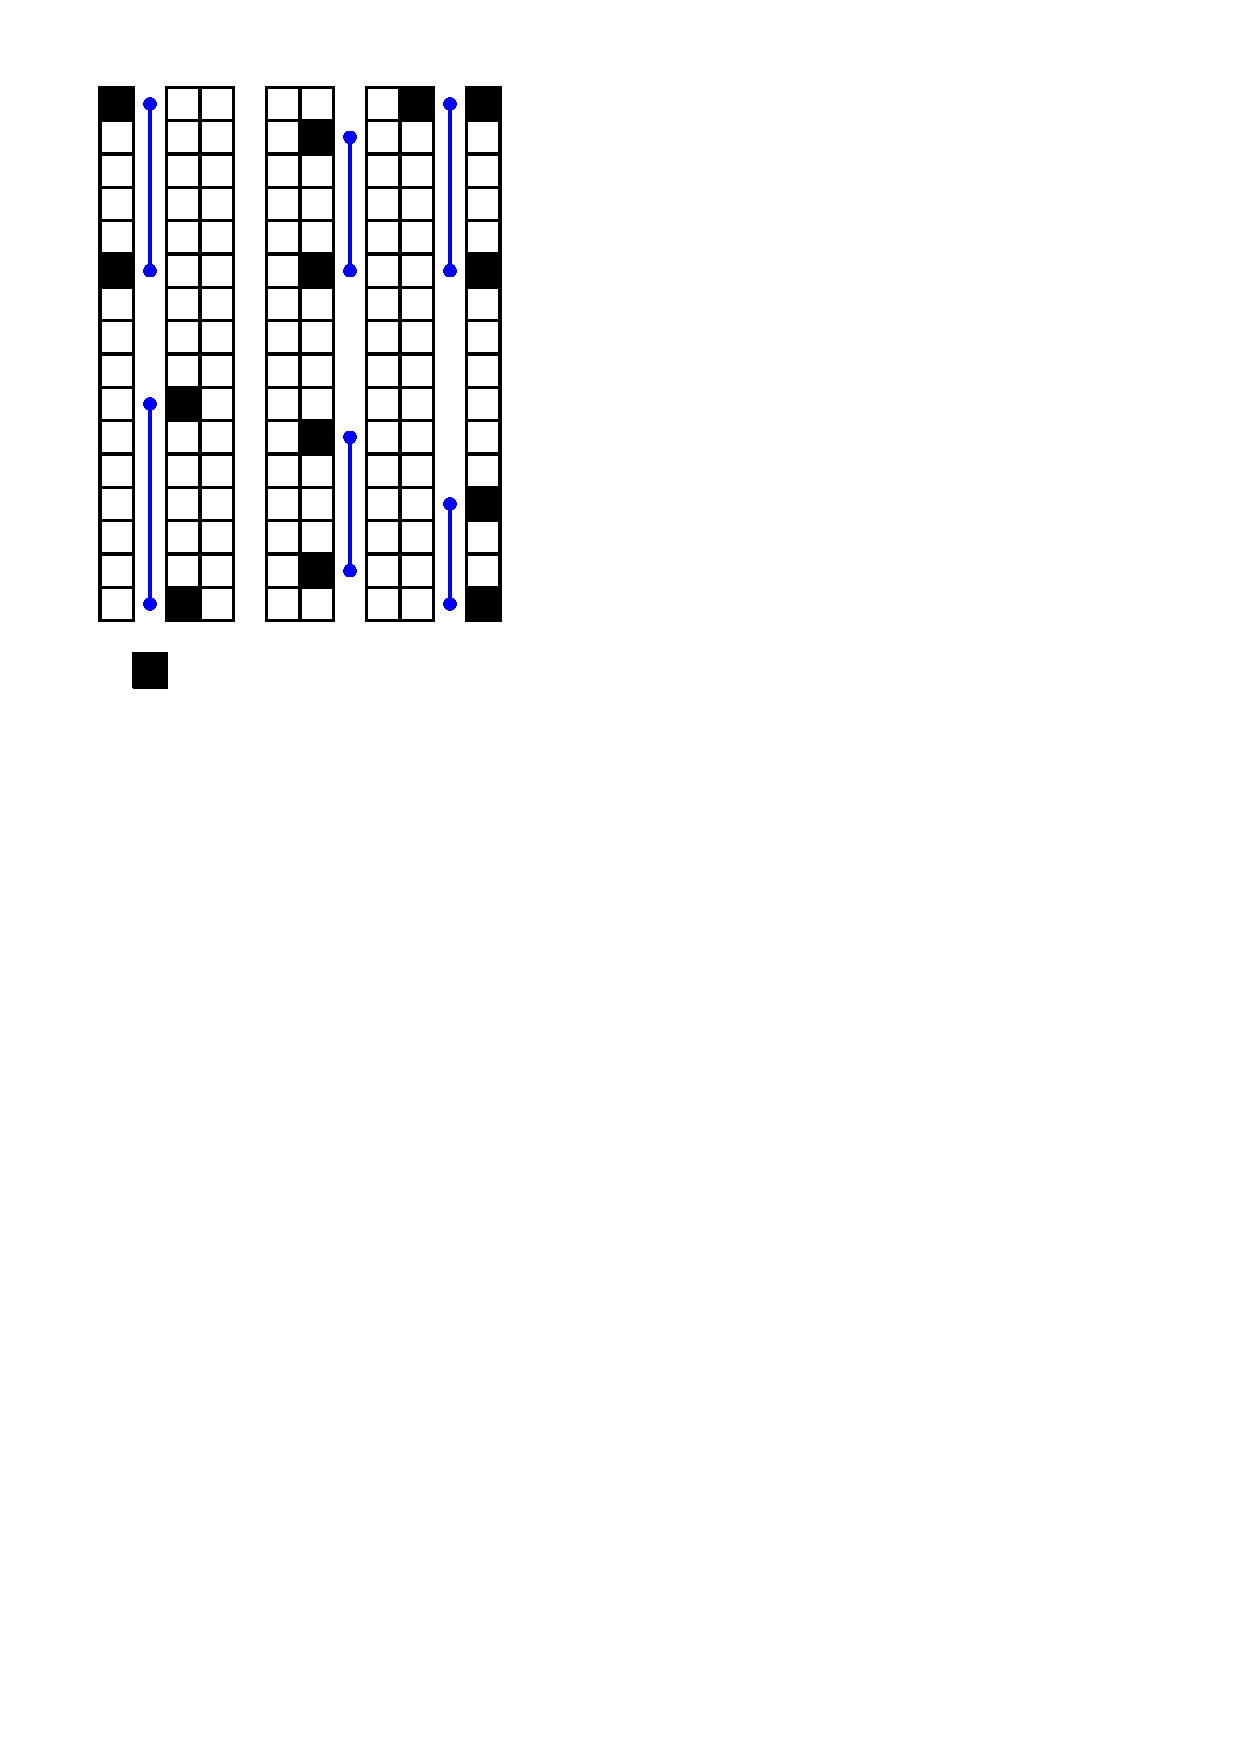
\includegraphics[width=0.8\linewidth]{discret_3}
				\end{figure}
				
	\end{minipage}}}%
	\hfill%
	
\end{frame}



\begin{frame}{Heur\'istica de corre\c{c}\~ao de rotas}
	
	\framesubtitle{(Discretiza\c{c}\~ao de pontos (SCHOLZ, et al. 2016))}
	\fboxsep=0pt
	Rotas do TSP podem ser infact\'iveis para o SPRP
	\noindent\fbox{%
		\begin{minipage}[t]{0.48\linewidth}
			\begin{itemize}
				\item[]
			\end{itemize}
			\begin{figure}			
				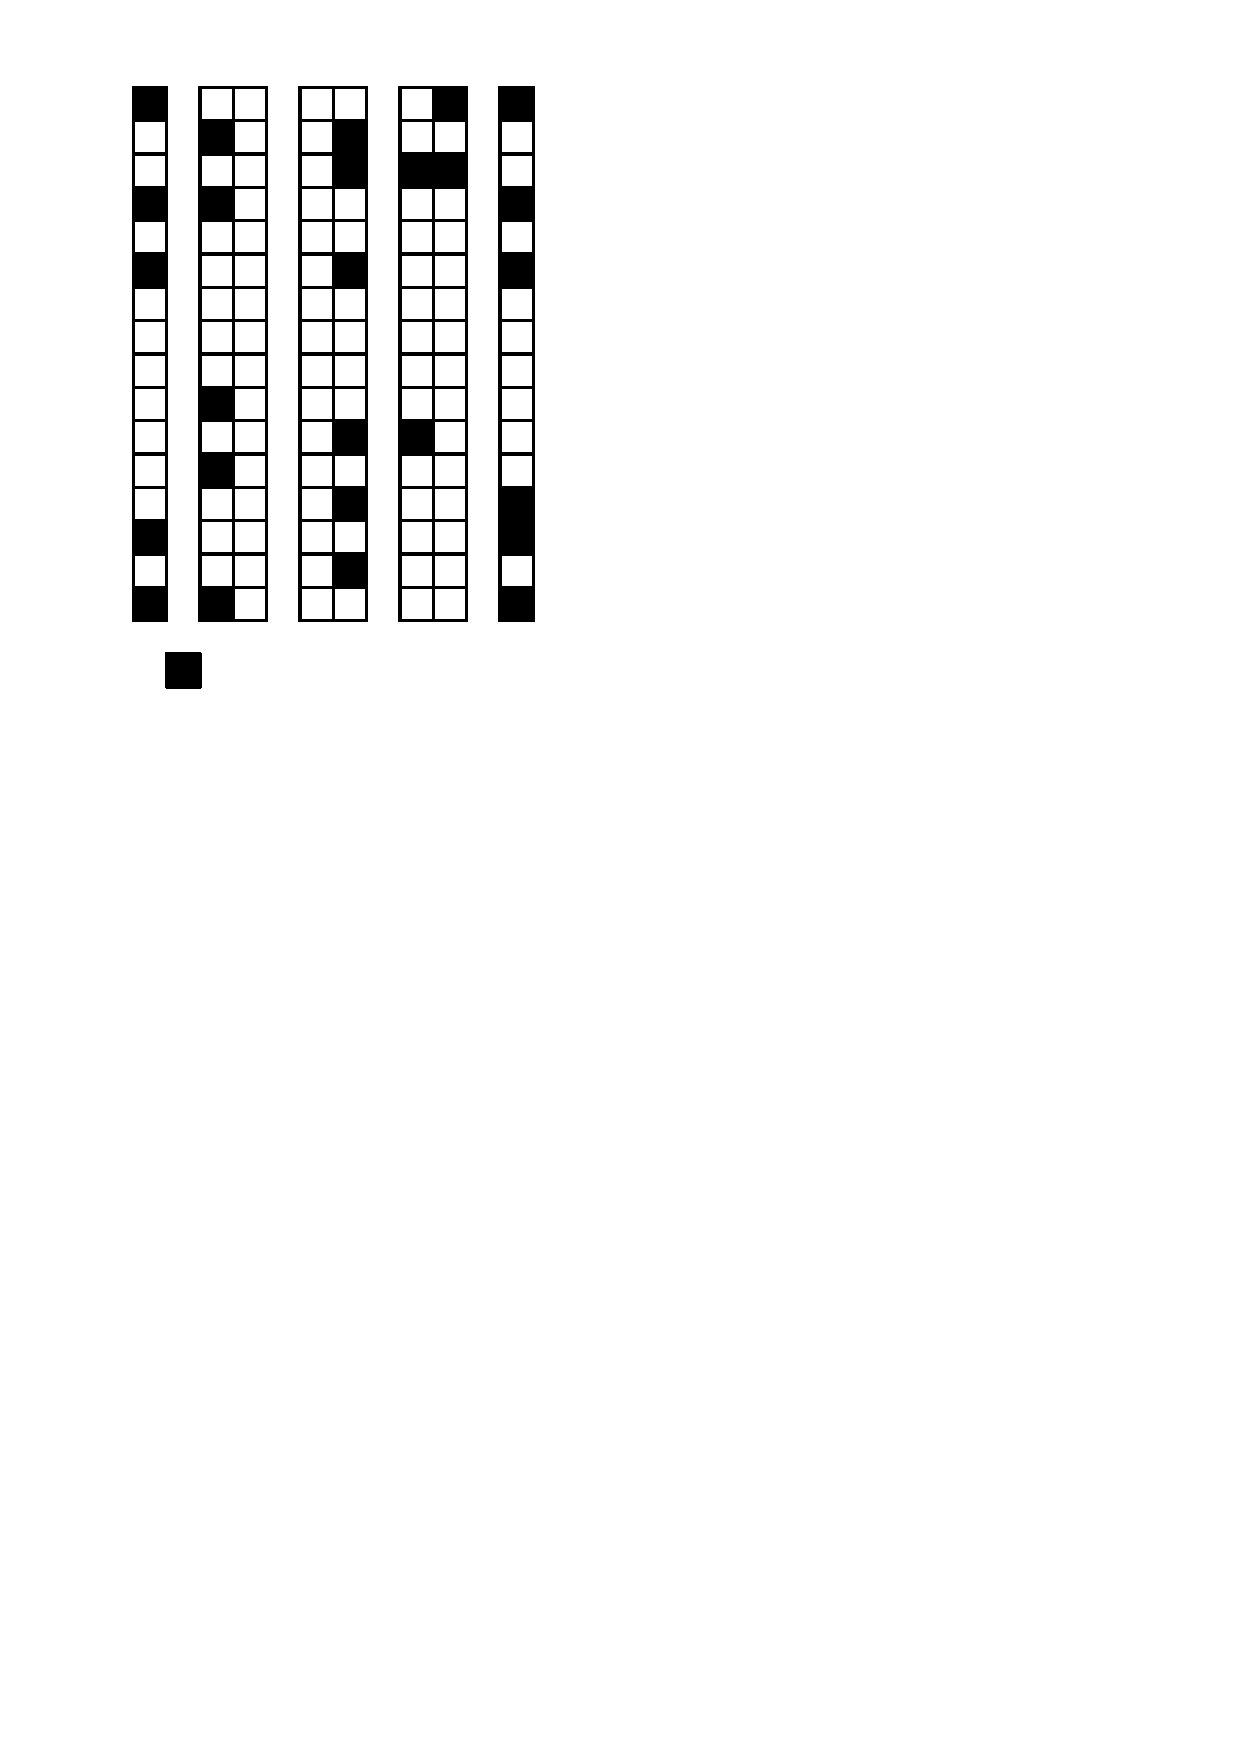
\includegraphics[width=0.8\linewidth]{discret_1}
			\end{figure}
			
	\end{minipage}}%
	\hfill%
	{%
		\noindent\fbox{%
	\begin{minipage}[t]{0.48\linewidth}
			\begin{itemize}
			\item[]
		\end{itemize}
		\begin{figure}			
			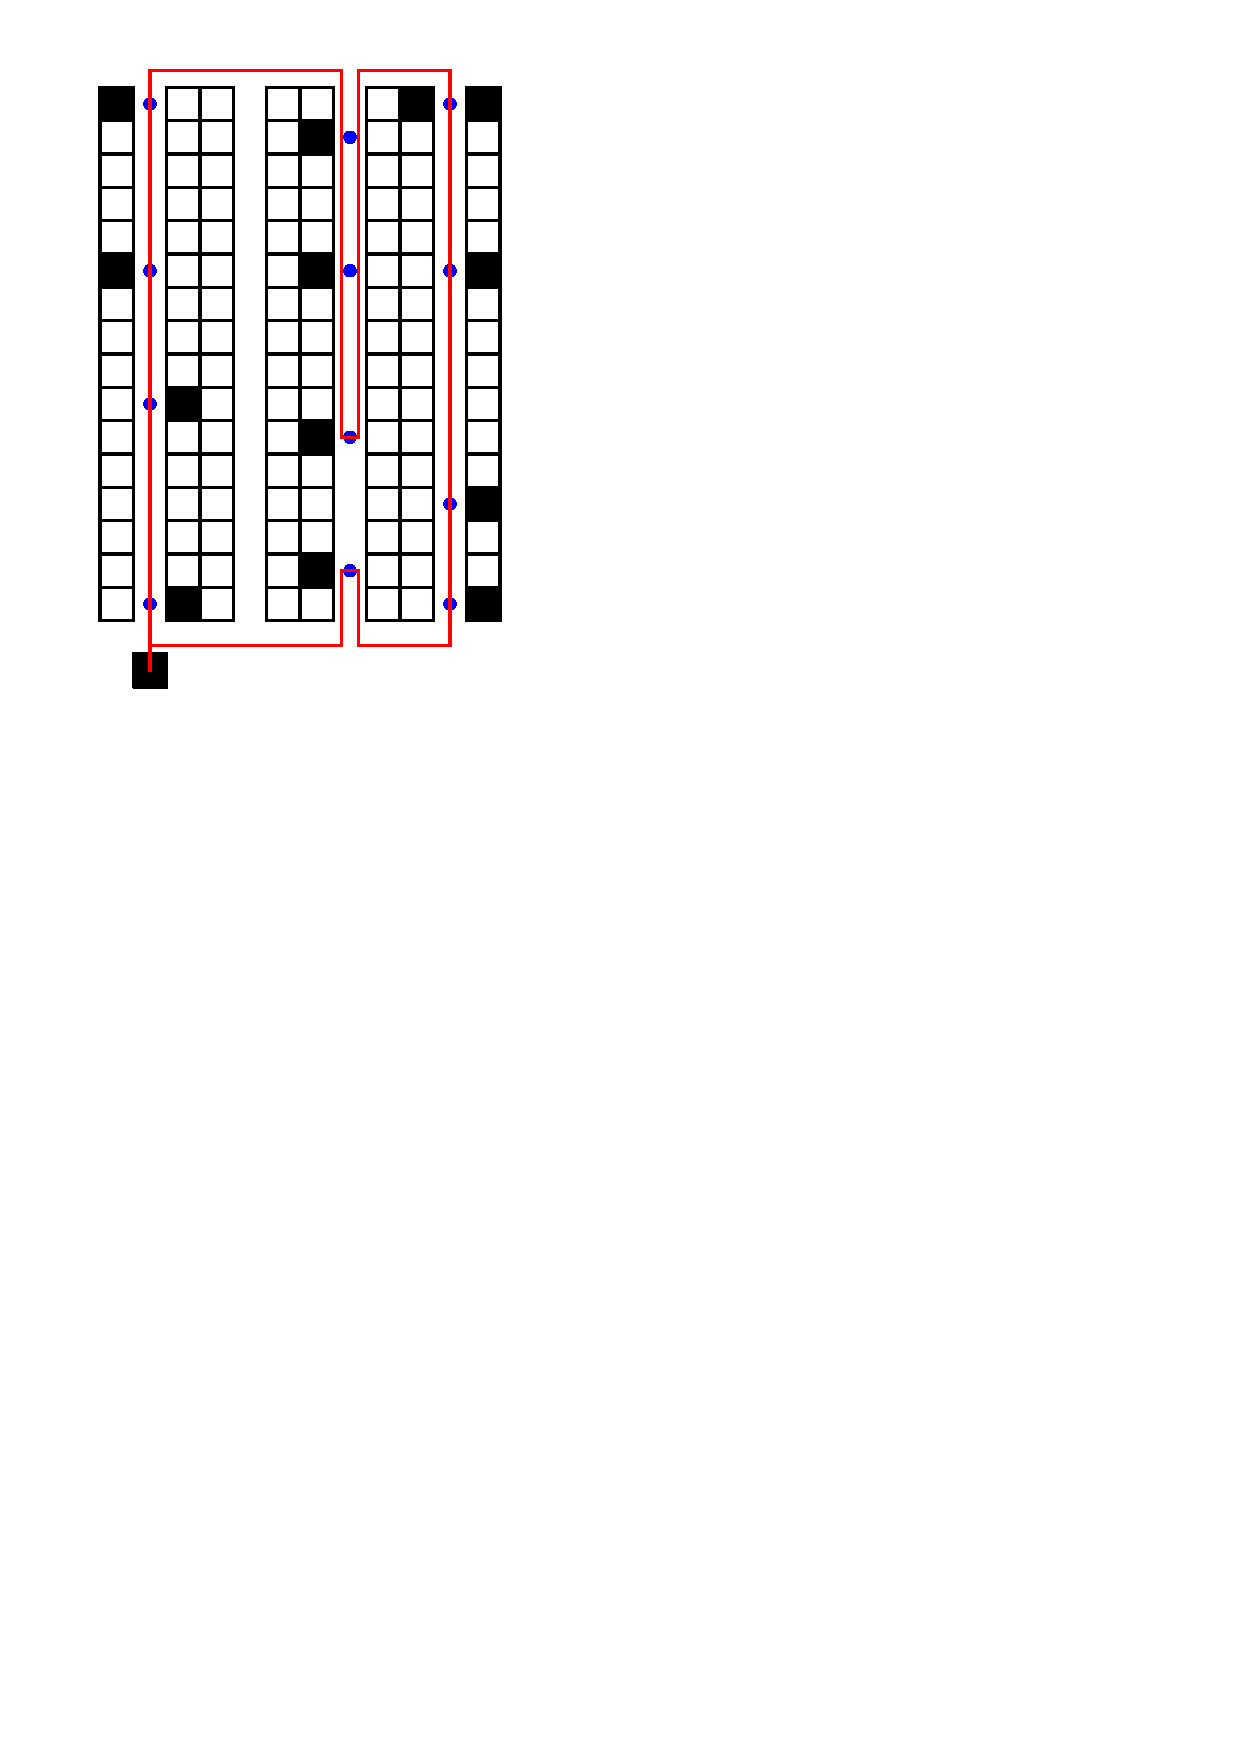
\includegraphics[width=0.8\linewidth]{sprp_infact}
		\end{figure}				
				
	\end{minipage}}}%
	\hfill%
	
\end{frame}

\begin{frame}{Heur\'istica de corre\c{c}\~ao de rotas}
	\framesubtitle{Passos}
	\begin{itemize}
		\item[\bfseries 1] {\bfseries Expans\~ao da \'arvore}
		\pause
		\item[\bfseries 2] {\bfseries Armazenamento de rotas fact\'iveis para o \textit{TSP} }
		\pause
		\item[\bfseries 3] {\bfseries Ordena\c{c}\~ao n\~ao decrescente em Z}
		\pause
		\item[\bfseries 4] {\bfseries Corre\c{c}\~ao das rotas infact\'iveis para o SPRP}
	\end{itemize}
\end{frame}

% Para fazer animações :
% 1-Salvar todas a imagens da animação em PDF
% Entrar no site https://ezgif.com/maker e criar um gif, de PDF para gif
% Entrar no site https://convertio.co/pt/ e transformar o GIF em PNG (se as imagens já estiverm em pnj não precisa fazer tudo isso, é porque o IPE não salva neste fomrmato)

\begin{frame}{Heur\'istica de corre\c{c}\~ao de rotas}
	\begin{enumerate}
		\item[1] Expans\~ao da \'arvore 
	\end{enumerate}
	\framesubtitle{(Expans\~ao da \'arvore)}
	\begin{figure}
 \animategraphics[height=2.4in,autoplay,controls]{1}{imagens_animacao_arvore2/388fbfde8e254523960540b1a6cc10af-}{0}{22}
  \end{figure}
\end{frame}

\begin{frame}{Heur\'istica de corre\c{c}\~ao de rotas}
	\begin{enumerate}
		\item[2] Armazenamento de rotas fact\'iveis para o TSP 
	\end{enumerate}
	\framesubtitle{(Expans\~ao da \'arvore)}
	\begin{figure}
		\animategraphics[height=2.4in,autoplay,controls]{1}{imagens_animacao_arvore2_coleta_bounds/2d8eb769d8e34a61a9b6387c3a461670-}{0}{8}
	\end{figure}
\end{frame}

\begin{frame}{Heur\'istica de corre\c{c}\~ao de rotas}
	\begin{enumerate}
		\item[3] Ordena\c{c}\~ao n\~ao decrescente em Z 
	\end{enumerate}
	\framesubtitle{(Ordena\c{c}\~ao n\~ao decrescente em Z)}
	\begin{figure}
		\animategraphics[height=2.4in,autoplay,controls]{1}{imagens_animacao_arvore2_sort/1f2f9d01ec8a46d6bccc1bf784fd0734-}{0}{9}
	\end{figure}
\end{frame}

\begin{frame}{Heur\'istica de corre\c{c}\~ao de rotas}
	\begin{enumerate}
		\item[4]  Corre\c{c}\~ao das rotas infact\'iveis para o SPRP 
	\end{enumerate}
	\framesubtitle{( Corre\c{c}\~ao das rotas infact\'iveis para o SPRP)}
		\begin{figure}			
	\includegraphics<1>[width=0.8\linewidth]{imagens_ordem_correcao/cor-0}
	\includegraphics<2>[width=0.8\linewidth]{imagens_ordem_correcao/cor-1}
	\includegraphics<3>[width=0.8\linewidth]{imagens_ordem_correcao/cor-2}
	\includegraphics<4>[width=0.8\linewidth]{imagens_ordem_correcao/cor-3}
	\includegraphics<5>[width=0.8\linewidth]{imagens_ordem_correcao/cor-4}
	\includegraphics<6>[width=0.8\linewidth]{imagens_ordem_correcao/cor-5}
       \end{figure}
\end{frame}

\begin{frame}{Heur\'istica de corre\c{c}\~ao de rotas}
\framesubtitle{( Corre\c{c}\~ao das rotas infact\'iveis para o SPRP)}

		Como identificar {\color{red}{\bfseries{rotas}}} infact\'iveis \ ?
		
\begin{center}
		\begin{figure}			
	
	    \includegraphics<1>[width=0.5\linewidth]{imagens_correcao/corr-1}
		\includegraphics<2>[width=0.5\linewidth]{imagens_correcao/corr-2}
		\includegraphics<3>[width=0.5\linewidth]{imagens_correcao/corr-3}
	\end{figure}
\end{center}
\end{frame}

\begin{frame}{Heur\'istica de corre\c{c}\~ao de rotas}
	Como identificar {\color{red}{\bfseries{arcos}}} infact\'iveis \ ?
	\framesubtitle{( Corre\c{c}\~ao das rotas infact\'iveis para o SPRP)}
\begin{center}
		\begin{figure}			
	
		\includegraphics<1>[width=0.5\linewidth]{imagens_correcao/corr-4}
		\includegraphics<2>[width=0.5\linewidth]{imagens_correcao/corr-5}
		\includegraphics<3>[width=0.5\linewidth]{imagens_correcao/corr-6}
		\includegraphics<4>[width=0.5\linewidth]{imagens_correcao/corr-7}
		\includegraphics<5>[width=0.5\linewidth]{imagens_correcao/corr-8}
		\includegraphics<6>[width=0.5\linewidth]{imagens_correcao/corr-9}
		\includegraphics<7>[width=0.5\linewidth]{imagens_correcao/corr-10}
		\includegraphics<8>[width=0.5\linewidth]{imagens_correcao/corr-11}
		\includegraphics<9>[width=0.5\linewidth]{imagens_correcao/corr-12}
		\includegraphics<10>[width=0.5\linewidth]{imagens_correcao/corr-13}
		\includegraphics<11>[width=0.5\linewidth]{imagens_correcao/corr-14}
	\end{figure}
\end{center}
\end{frame}

\begin{frame}{Heur\'istica de corre\c{c}\~ao de rotas}
	Ao inv\'es de identificar oa arcos {\color{red}{\bfseries{infact\'iveis}}} , identificar os {\color{blue}{\bfseries{fact\'iveis}}} 
	\framesubtitle{( Corre\c{c}\~ao das rotas infact\'iveis para o SPRP)}
	\begin{center}
		\begin{figure}			
			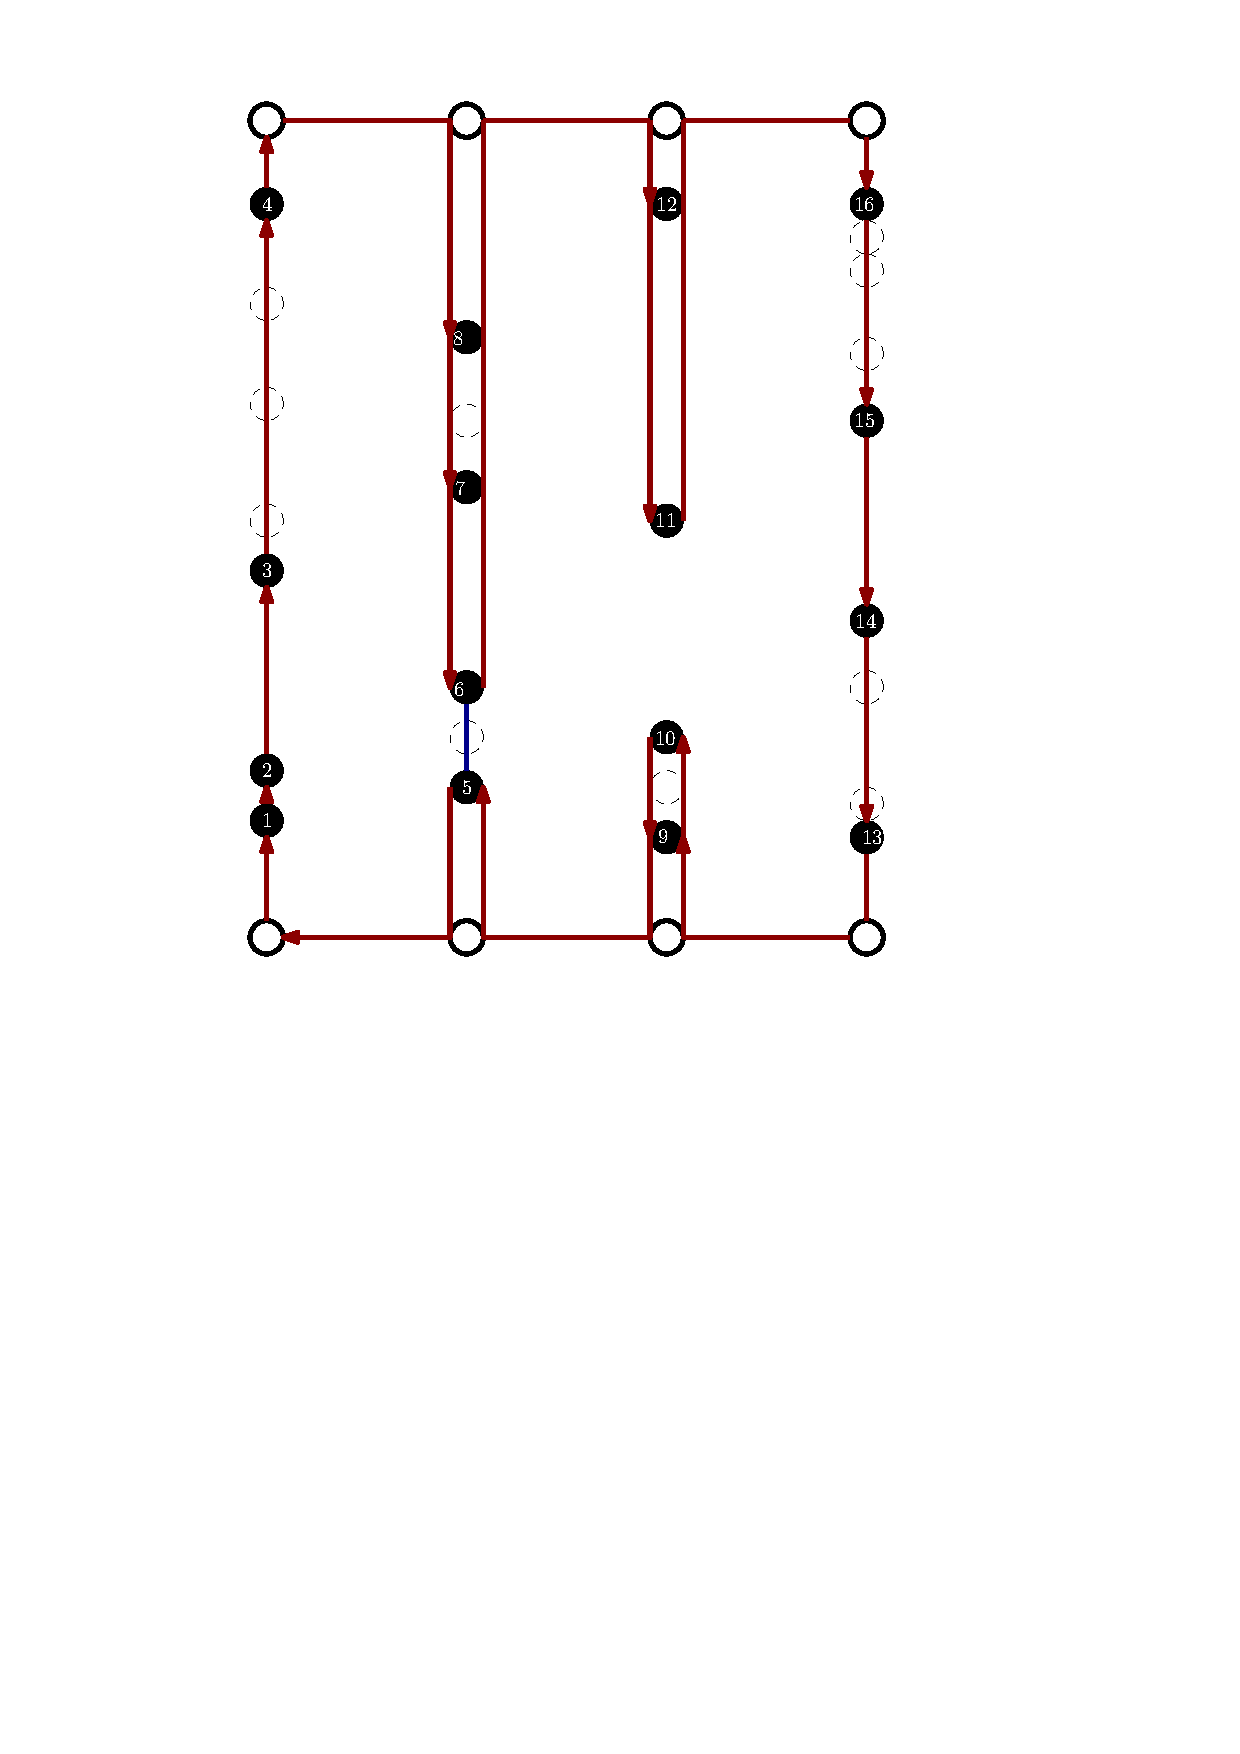
\includegraphics[width=0.5\linewidth]{imagens_correcao/corr-14}
		\end{figure}
	\end{center}
\end{frame}

\begin{frame}{Heur\'istica de corre\c{c}\~ao de rotas}
	\framesubtitle{( Corre\c{c}\~ao das rotas infact\'iveis para o SPRP)}
	\fboxsep=0pt
	\noindent{%
		\begin{minipage}[t]{0.6\linewidth}
			\begin{figure}			
		\includegraphics<1>[width=0.8\linewidth]{imagens_correcao/corr-15}
		\includegraphics<2>[width=0.8\linewidth]{imagens_correcao/corr-16}
		\includegraphics<3>[width=0.8\linewidth]{imagens_correcao/corr-17}
		\includegraphics<4>[width=0.8\linewidth]{imagens_correcao/corr-18}
		\includegraphics<5>[width=0.8\linewidth]{imagens_correcao/corr-19}
		\includegraphics<6>[width=0.8\linewidth]{imagens_correcao/corr-20}
		\includegraphics<7>[width=0.8\linewidth]{imagens_correcao/corr-21}
		\includegraphics<8>[width=0.8\linewidth]{imagens_correcao/corr-22}
		\includegraphics<9>[width=0.8\linewidth]{imagens_correcao/corr-23}
\end{figure}
			
	\end{minipage}}%
	\hfill%
	{%
		\begin{minipage}[t]{0.4\linewidth}
			\begin{itemize}
			    {\normalsize 	\item Identifica\c{c}\~ao dos pontos por corredor}
				\pause
				\item Identificar a ordem (1,2,3 ou 4) em que os pontos (P1,P2) se ligam e se a liga\c{c}\~ao \'e realizada por baixo ou por cima
			

			\end{itemize}
		\end{minipage}
	}
\end{frame}

\begin{frame}{Heur\'istica de corre\c{c}\~ao de rotas}
	\framesubtitle{( Corre\c{c}\~ao das rotas infact\'iveis para o SPRP)}
	\fboxsep=0pt
	\noindent{%
	\begin{minipage}[t]{0.6\linewidth}
		\begin{figure}			
	      \includegraphics<1>[width=0.9\linewidth]{imagens_correcao/corr-24}
	      \includegraphics<2>[width=0.9\linewidth]{imagens_correcao/corr-25}
	      \includegraphics<3>[width=0.9\linewidth]{imagens_correcao/corr-30}
	      \includegraphics<4>[width=0.9\linewidth]{imagens_correcao/corr-27}
	      \includegraphics<5>[width=0.9\linewidth]{imagens_correcao/corr-28}
	      \includegraphics<6>[width=0.9\linewidth]{imagens_correcao/corr-29}
\end{figure}
			
	\end{minipage}}%
	\hfill%
	{%
		\begin{minipage}[t]{0.4\linewidth}
			\begin{itemize}
				\item Remover o arco do meio (nunca haver\'a itens)
				\pause
				\item Inserir o arco obrigat\'orio
				\pause
				\item Identificar arcos a serem removidos e inseridos
				\pause
				\item Remover os arcos do centro
				\pause
				\item Inserir o arco obrigat\'orio
			\end{itemize}
		\end{minipage}
	}
\end{frame}


%%%%%%%%%%%%%%%%%%%%%%%%%%%%%%%%%%%%%%%%%%%%%%%%%%%%%%%%%%%%%%%%%%%%%%%%%%%%%%%%%%%%%
\section{Heur\'istica de Empacotamento} %
	\begin{frame}[shrink]{Heur\'istica de Empacotamento} %reduz o tamanho do frame para que tudo caiba em um 
		\footnotesize
	\framesubtitle{( Dados do Problema}
	{\bfseries Dados:}
    \begin{itemize}  	
    	\item Uma lista de caixas diferentes, com suas dimensões (x,y,z), suas massas e  massas m\'aximas
    	\item Uma sequ\^encia com tipos e quantidades de caixas
    	\item Um objeto com dimens\~oes (X,Y,Z)  	
    \end{itemize}
	{\bfseries Objetivo:}
	   \begin{itemize}		
		\item M\'aximizar o n\'umero de caixas alocadas no objeto, de tal forma que:

			\begin{itemize}			
			\item[1]<1->  N\~ao exista sobreposi\c{c}\~ao
			\item[2]<2-> Todos as caixas estejam totalmente dentro do objeto	
			\item[3]<3-> Todos as caixas estejam totalmente dentro do objeto
			\item[4]<4-> A base de todas as caixas esteja totalmente apoiada
			\item[5]<5-> As caixas sejam alocadas na ordem da lista
			\end{itemize} 	
	\end{itemize}
\end{frame}

\begin{frame}{Heur\'istica de Empacotamento} %reduz o tamanho 
	\framesubtitle{(Passos)}

	\begin{itemize}
		\item  Heur\'istica recursiva, com base em cria\c{c}\~ao e consumo de espa\c{c}os
	\end{itemize}
	
	\pause
	\begin{algorithm}[H]
		\SetAlgoLined
		\While{caixas != 0 e espa\c{c}o != 0}{
			encontrar espa\c{c}o\;
			inserir caixa no espa\c{c}o\;
			gerar novos espa\c{c}o\;
			atualizar quantidades de espa\c{c}o e caixas\;			
		}
		\caption{Empacotamento}
	\end{algorithm}
\end{frame}



\begin{frame}{Heur\'istica de Empacotamento}
	\framesubtitle{( Corre\c{c}\~ao das rotas infact\'iveis para o SPRP)}
	\fboxsep=0pt
	\noindent{%
		\begin{minipage}[t]{0.48\linewidth}
		
		\begin{figure}			
			\includegraphics<1->[width=0.9\linewidth]{objeto}
        \end{figure}
    	\begin{itemize}
    	\item Objeto
       \end{itemize}
	    \end{minipage}}%
	\hfill%
	{%
		\begin{minipage}[t]{0.48\linewidth}
		\begin{figure}			
			\includegraphics<2->[width=0.9\linewidth]{objeto_caixa}
		\end{figure}
		\begin{itemize}
		\item<2-> Objeto com primeira caixa alocada
	    \end{itemize}
		\end{minipage}
	}
\end{frame}

\begin{frame}{Heur\'istica de Empacotamento}
	\framesubtitle{(Gera\c{c}\~ao de espa\c{c}os)}
	\fboxsep=0pt
	\noindent{%
		\begin{minipage}[t]{0.6\linewidth}
			
			\begin{figure}			
				\includegraphics<1>[width=0.9\linewidth]{inser_1}
				\includegraphics<2>[width=0.9\linewidth]{inser_2}
				\includegraphics<3>[width=0.9\linewidth]{inser_3}
				\includegraphics<4>[width=0.9\linewidth]{inser_4}
				\includegraphics<5>[width=0.9\linewidth]{inser_5}
			\end{figure}
	
	\end{minipage}}%
	\hfill%
	{%
		\begin{minipage}[t]{0.35\linewidth}
			\begin{figure}			
				\includegraphics<1>[width=0.9\linewidth]{graf_1}
				\includegraphics<2>[width=0.9\linewidth]{graf_2}
				\includegraphics<3>[width=0.9\linewidth]{graf_3}
				\includegraphics<4>[width=0.9\linewidth]{graf_4}
				\includegraphics<5>[width=0.9\linewidth]{graf_5}
			\end{figure}
		\end{minipage}
	}
\end{frame}

\begin{frame}{}

\end{frame}

\begin{frame}{Heur\'istica de Empacotamento}
			\begin{figure}
			\framesubtitle{(Exemplo de carregamento)}			
	\includegraphics<1>[width=1\linewidth]{caix_arv_1}
	\includegraphics<2>[width=1\linewidth]{caix_arv_2}
	\includegraphics<3>[width=1\linewidth]{caix_arv_3}
	\includegraphics<4>[width=1\linewidth]{caix_arv_4}
	\includegraphics<5>[width=1\linewidth]{caix_arv_5}
\end{figure}
\end{frame}


\section{Heur\'istica de Escoamento de Pontos (H.E.P)} %
	\begin{frame}{Heur\'istica de Escoamento de Pontos (H.E.P)}
\end{frame}
\section{Resultados} %
	\begin{frame}{Resultados}
\end{frame}

	
	
	
	
\end{document} 